\documentclass[11pt,a4paper]{article}
\usepackage[margin=22mm]{geometry}
\usepackage{graphicx}
\usepackage{amsmath,amssymb}
\usepackage{booktabs}
\usepackage{siunitx}
\usepackage{microtype}
\usepackage[hidelinks]{hyperref}
\usepackage{caption}
\usepackage{authblk}
\usepackage{xcolor}
\usepackage[numbers,sort&compress]{natbib}
\captionsetup{font=small,labelfont=bf}
\sisetup{per-mode=symbol,separate-uncertainty=true,range-phrase=--,range-units=single,retain-explicit-plus=true}
\graphicspath{{figures/}}
\newcommand{\ChronoFlow}{ChronoFlow}
\newcommand{\dd}{\mathrm{d}}

\title{\ChronoFlow: an electricity-free, volumetric, clockwork-governed syringe infusion driver for neonatal care in low-resource settings}
\author[1]{Author list to be completed}
\affil[1]{Affiliation to be completed}
\date{Design-and-simulation study --- \today}

\begin{document}
\maketitle

\begin{abstract}
Hospitals without reliable electricity deliver intravenous fluids and drugs to newborns by gravity drip or by hand. The only non-electric infusion devices available meter flow by pushing fluid through a restriction, so the delivered rate depends on fluid viscosity (temperature, drug) and on downstream pressure; low-cost electric pumps still need batteries and cost hundreds of dollars. We present \ChronoFlow, a wind-up syringe driver that meters \emph{volume} rather than pressure: a constant-force spring pushes the plunger and a rack-and-pinion drives a 3D-printed step-up gear train into a clockwork escapement whose balance wheel sets the rate. Two design problems were identified and solved by simulation. First, the mechanical power available to the escapement varies $24\times$ across syringe sizes, clinical rates and loads (\SIrange{17}{416}{\micro\watt}); a conventional lever escapement, whose impulse scales with train torque, over-banks over most of this range. Adapting the gravity-escapement principle of tower clocks with springs---a constant-force \emph{spring-arm} escapement---delivers a fixed impulse energy per beat and holds the balance amplitude constant over the full range with a period error below \SI{0.06}{\percent}. Second, a cross-spring flexure pivot was shown by a beam-column finite-element model to change stiffness by \SI{17}{\percent} under the balance's own weight; it was replaced by a taut-band torsion suspension made from \SI{0.0015}{in} (\SI{38.1}{\micro\metre}) feeler-gauge steel ribbon, giving a \SI{1.20}{\hertz} balance with \SI{\pm 0.19}{\percent} orientation sensitivity and no pivot friction. Colour-coded gear cassettes provide 1, 2, 5 and \SI{10}{\milli\litre\per\hour} on a \SI{20}{\milli\litre} syringe (\SIrange{0.4}{19.5}{\milli\litre\per\hour} across 5--\SI{60}{\milli\litre} syringes) at \SIrange{0.12}{1.16}{\micro\litre} per beat. A 20\,000-sample Monte-Carlo error budget predicts that \SI{95}{\percent} of units deliver within \SI{\pm 1.14}{\percent} of the set rate, compared with \SI{+45}{\percent} at \SI{37}{\celsius} and \SI{-33}{\percent} at \SI{100}{mmHg} back-pressure for flow-restriction pumps. A trip spring whose preload is keyed to the syringe size stops the oscillator and raises a flag at \SI{300}{mmHg} occlusion (280--320 to 202--\SI{398}{mmHg} across syringe sizes once plunger-friction uncertainty is included) and a syringe-latch interlock prevents free-flow boluses. The complete 91-part assembly was modelled parametrically, checked for interferences and exported for printing; the bill of materials is \$40. No physical prototype has yet been built; a bench protocol following IEC~60601-2-24~\cite{iec} is provided.
\end{abstract}

\section{Introduction}
Neonates require maintenance fluids at \SIrange{60}{100}{\milli\litre\per\kilo\gram\per\day} and drugs such as antibiotics, dextrose and inotropes at \SIrange{0.5}{10}{\milli\litre\per\hour}; a \SI{10}{\percent} rate error or an uncontrolled bolus of a few millilitres is clinically significant. Electronic syringe pumps meet this need where mains power, batteries and service infrastructure exist. Where they do not, three alternatives have been described. Low-cost electro-mechanical pumps such as AutoSyP combine a constant-force spring with a motor and battery and reach \SI{\pm 4}{\percent} accuracy at a cost of goods of about \$500~\cite{autosyp}. Non-electric flow-restriction devices (elastomeric pumps, the Springfusor, and an adjustable air-over-oil design~\cite{asme2017}) obey $Q \propto \Delta P/\mu$ and therefore drift with fluid viscosity, temperature and back-pressure. Clockwork metering has been reported four times: a gravity-driven neonatal driver regulated by a pendulum metronome, which must sit level and still~\cite{asme2011}; a wind-up kitchen-timer movement adapted for microfluidics~\cite{han2021} and its fully 3D-printed successor with a hairspring balance~\cite{park2024snb,park2024hx}, both with fixed rates set by gear choice and about an hour of running time; and a spring-driven leadscrew pump whose escapement is actuated electrically for insulin dosing~\cite{pooke2023}.

The gap is a non-electric device that meters \emph{volume}, works in any orientation, offers selectable clinical rates, runs for a full syringe without re-winding and has mechanical occlusion detection and free-flow protection. \ChronoFlow\ addresses it by returning to two solutions from precision mechanics: the constant-force escapement, introduced by Denison for tower clocks whose train torque varied with wind and ice on the hands~\cite{denison}, and the taut-band suspension of galvanometers, which removes pivot friction and most positional error.

\section{Design}
\subsection{Architecture and metering principle}
Figure~\ref{fig:overview}a--b shows the machine. Two constant-force springs (\SI{44.5}{\newton} total, $2\times\SI{5}{lbf}$) pull a carriage toward the syringe nozzle. The plunger load---syringe friction of \SIrange{1.5}{4.5}{\newton} plus pressure times bore area, up to \SI{26.9}{\newton} for a \SI{60}{\milli\litre} syringe at the \SI{300}{mmHg} trip---absorbs part of this force; the excess back-drives a module-1 rack and 12-tooth pinion through a $5\times5\times5\times2.5 = 312.5$ step-up train and a plug-in rate cassette to a 15-tooth escape wheel. The escapement releases one half-tooth per beat of the balance, so the plunger advance per beat is fixed by geometry:
\begin{equation}
\Delta x = \frac{\pi m z_0}{2 Z_e\, N_{\mathrm{fixed}}\, r_{\mathrm{c}}} = \frac{\pi \cdot 1 \cdot 12}{2\cdot 15 \cdot 312.5 \cdot r_{\mathrm{c}}}\ \si{\milli\metre},
\end{equation}
which is \SI{4.0}{\micro\metre} (\SI{1.16}{\micro\litre} on a BD \SI{20}{\milli\litre} syringe) for the unity cassette. Because the metered quantity is displacement, viscosity, temperature and downstream pressure do not enter the rate until the occlusion trip point (Fig.~\ref{fig:overview}c--d). The spring force is constant over the \SI{95}{\milli\metre} travel, so runtime is set only by syringe volume (2--\SI{20}{\hour} per \SI{20}{\milli\litre} fill) and the device never needs re-winding mid-infusion. A one-way click on the rack-pinion shaft lets the carriage be pulled back freely, so loading a syringe \emph{is} the winding action (\SI{4.2}{\joule} stored, about eleven times the \SI{0.37}{\joule} the escapement dissipates in \SI{20}{\hour}).

\begin{figure}[t]
\centering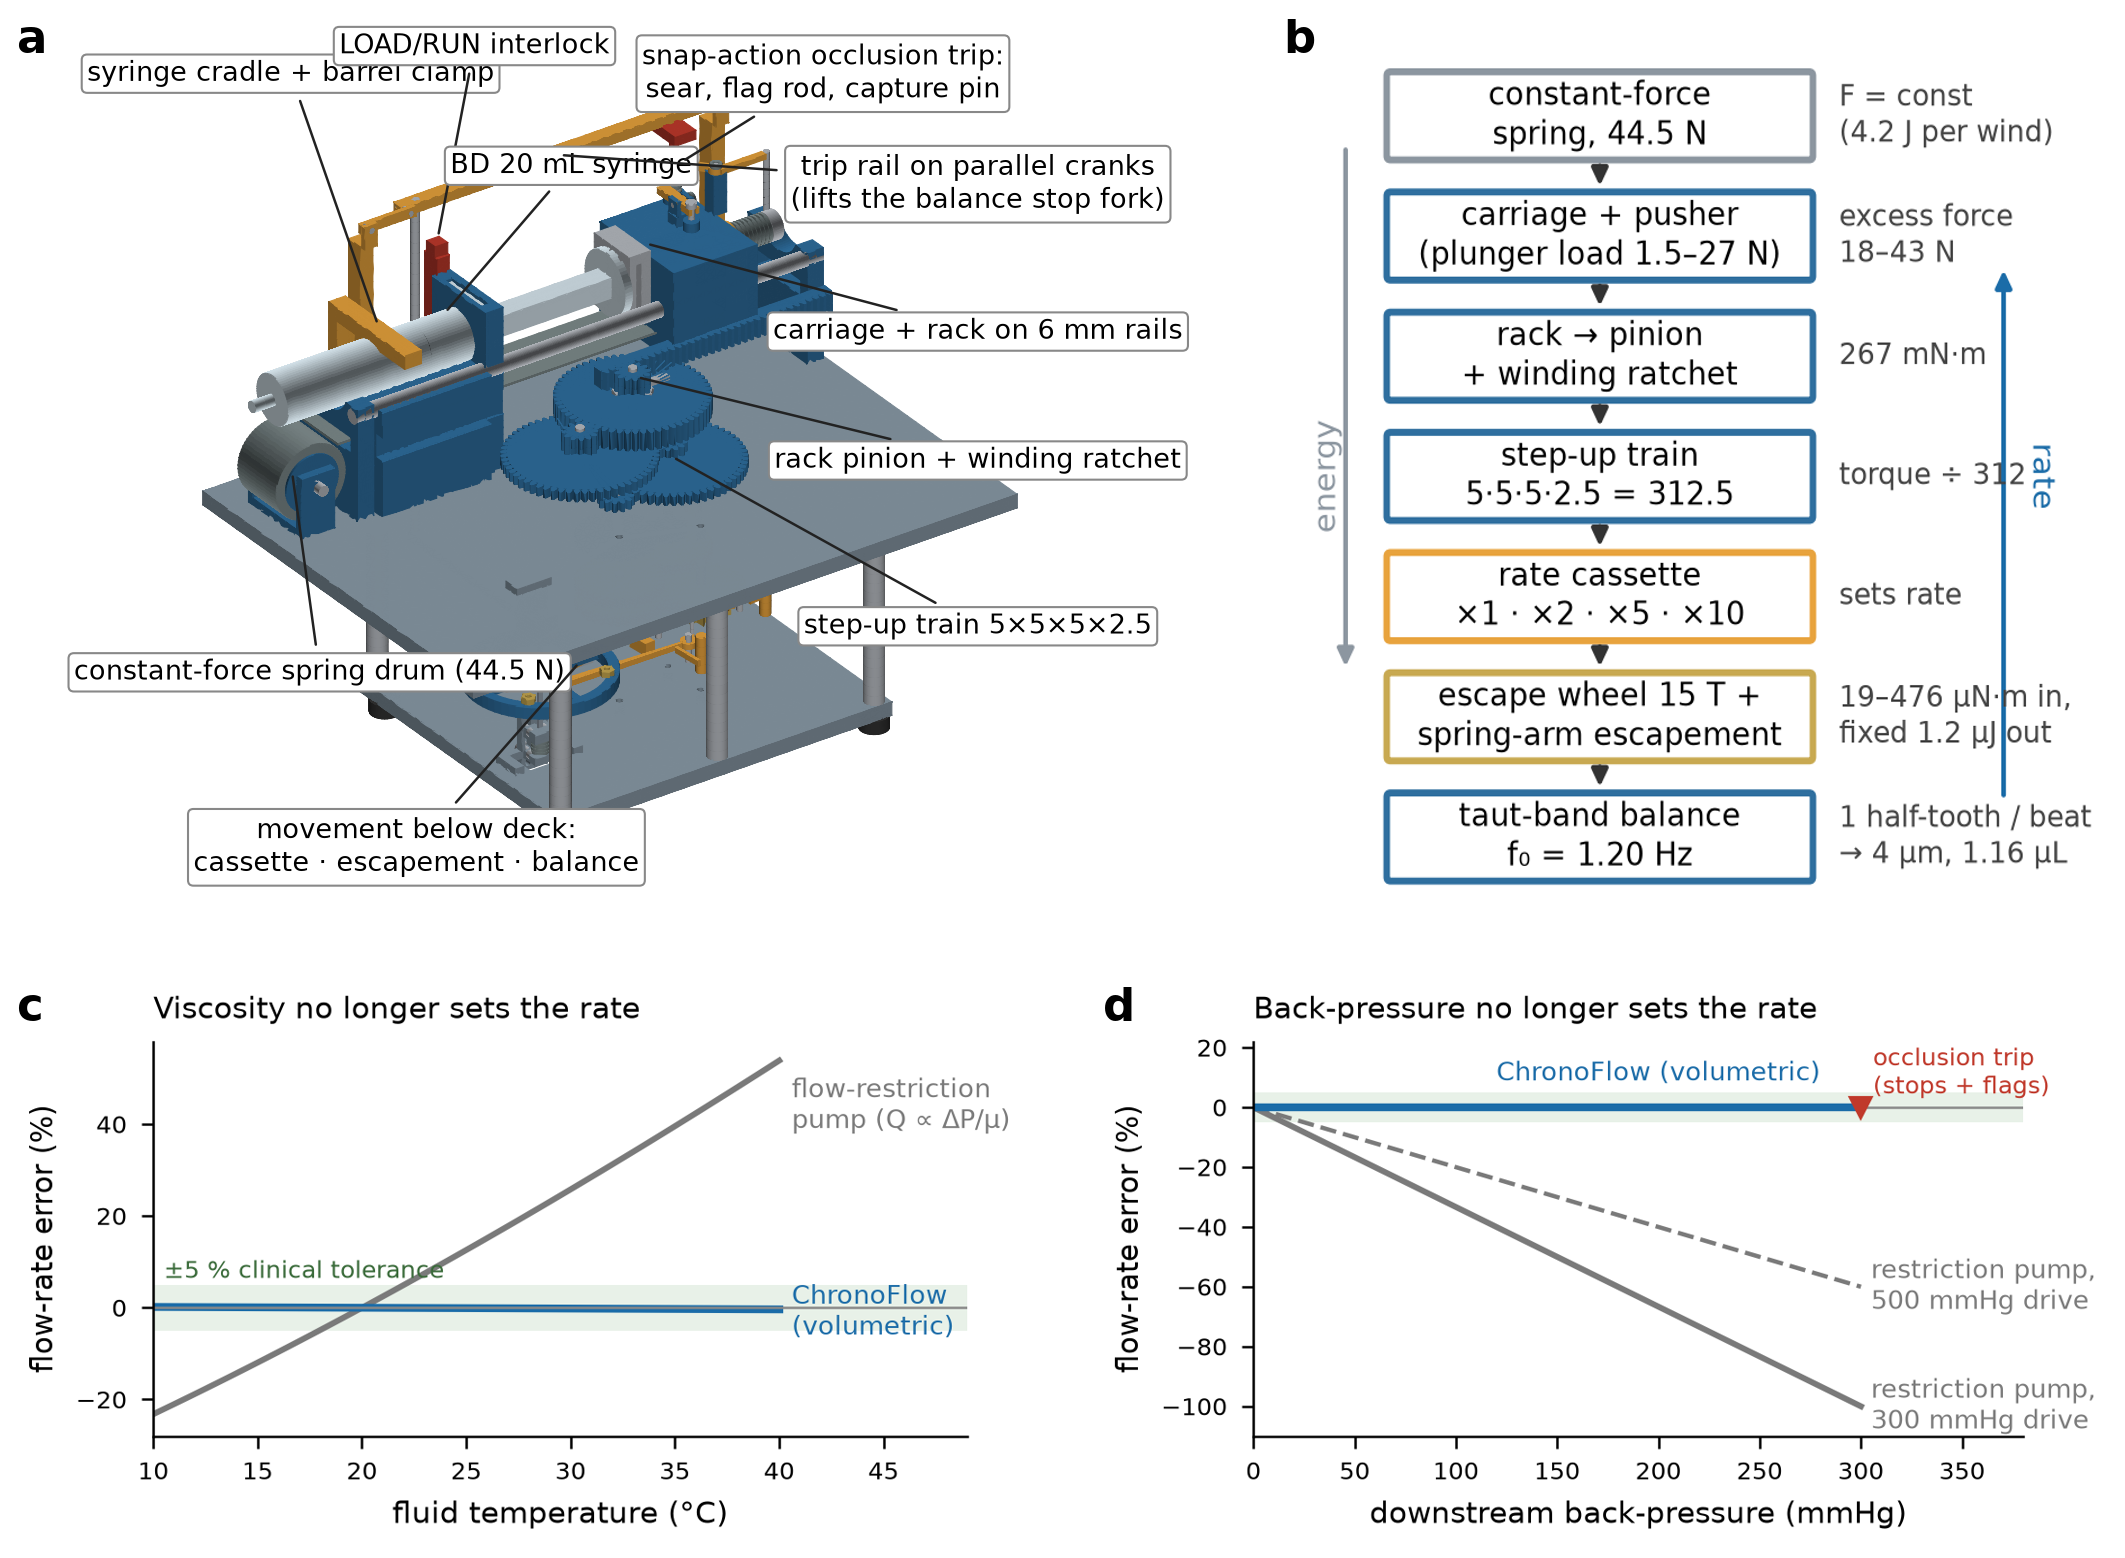
\includegraphics[width=\textwidth]{fig1.png}
\caption{\textbf{A spring-driven, clockwork-governed syringe driver meters volume, so the delivered rate is independent of fluid temperature and back-pressure.} (a) Labelled render of the parametric CAD assembly with a BD \SI{20}{\milli\litre} syringe at \SI{85}{\percent} fill and the \SI{10}{\milli\litre\per\hour} cassette. (b) Energy and metering chain; the left arrow follows energy from the spring to the balance, the right arrow follows the rate constraint back from the balance to the plunger. (c) Steady-state flow error versus fluid temperature for a flow-restriction pump calibrated at \SI{20}{\celsius} (water viscosity from the Vogel equation) and for \ChronoFlow\ (oscillator temperature coefficient $-1.8\times10^{-4}\,\mathrm{K}^{-1}$). (d) Flow error versus downstream back-pressure; \ChronoFlow\ stops and flags at the \SI{300}{mmHg} trip point. Green band: \SI{\pm 5}{\percent} clinical tolerance.}
\label{fig:overview}
\end{figure}

\subsection{Constant-force spring-arm escapement}
Power delivered to the escapement is $P = F_{\mathrm{excess}}\,v$. With $F_{\mathrm{excess}}$ between \SI{17.6}{\newton} (\SI{60}{\milli\litre} syringe at its \SI{300}{mmHg} occlusion trip) and \SI{43.0}{\newton} (free-running \SI{5}{\milli\litre} syringe) and $v$ spanning the 1--\SI{10}{\milli\litre\per\hour} cassettes, $P$ ranges from \SI{17}{\micro\watt} to \SI{416}{\micro\watt}; after a train efficiency of $0.95\times0.92^{6} = 0.58$ (seven meshes in total: the rack mesh at 0.95 and six printed gear meshes at 0.92---four step-up, two cassette; the escape wheel shares the cassette output shaft) the escape-wheel torque spans \SIrange{19}{476}{\micro\newton\metre}, a $24\times$ range. In a lever escapement the impulse energy delivered to the balance is proportional to this torque, so the balance amplitude scales as $\sqrt{T_e}$; our dynamic model (Section~\ref{sec:methods}) shows it exceeding the \SI{1.2}{\radian} banking limit over most of the operating range (Fig.~\ref{fig:escapement}b--c). Stalling at the low end or over-banking at the high end are both failures of rate.

The spring-arm escapement (Fig.~\ref{fig:escapement}a) separates the two energy flows. Each escape-wheel tooth \emph{cocks} one of two impulse arms against a printed flexure until a latch engages (phases 1--2). The train is then locked and any excess torque simply sits on the lock. When the balance passes, its impulse pin trips the latch (phase 3) and the arm delivers a fixed energy $E_{\mathrm{imp}} = \SI{1.2}{\micro\joule}$ over a \SI{15}{\degree} arc; the wheel then advances one half-pitch, re-cocks the opposite arm and relocks, the surplus train energy being dissipated in the locking impact. Train torque only has to exceed the re-cock minimum $T_{\min} = E_{\mathrm{imp}}/(\eta_{\mathrm{lift}}\,\pi/Z_e) = \SI{9.5}{\micro\newton\metre}$. The simulation confirms constant amplitude (\SI{0.59}{\radian} at $Q=150$) and a period error of \SI{0.06}{\percent} from the slightly asymmetric impulse window across the whole torque range (Fig.~\ref{fig:escapement}c--d). Because the balance's air damping cannot be known before a prototype exists, $Q$ was swept from 40 to 800: amplitude settles between \SI{0.31}{} and \SI{0.99}{\radian} and the period error between \SI{0.45}{} and \SI{0.01}{\percent} (Fig.~\ref{fig:escapement}e), a fixed offset that trim calibration absorbs.

The beat-level model takes $E_{\mathrm{imp}}$ and the latch cost as given; a mechanism-level analysis (Fig.~\ref{fig:arm}, \texttt{analysis\_arm\_mechanism.py}) derives both from the drawn geometry and follows the escape wheel through a beat. The arm (pivot-to-pallet \SI{5}{\milli\metre}, pivot-to-tip \SI{59}{\milli\metre}) pushes the impulse pin \SI{1.6}{\milli\metre}, so it unwinds by only \SI{27}{\milli\radian} per beat; with a pre-loaded torsion spring of $k = \SI{1e-4}{\newton\metre\per\radian}$ set at \SI{25}{\degree} the tip force is \SI{0.74}{\milli\newton}, the force droop over the impulse arc is \SI{6}{\percent} (the sense in which the impulse is ``constant''), a \SI{0.1}{\milli\metre} latch-position tolerance biases $E_{\mathrm{imp}}$ by \SI{1.4}{\percent} once per build, and beat-to-beat scatter of the release point (\SI{5}{\micro\metre}) changes it by \SI{0.07}{\percent}. A printed \SI{0.8}{\milli\metre} flexure is too soft for this preload (it would need \SI{2.9}{\radian}), so the arm spring is specified as music wire rather than as the printed flexure of earlier revisions. Unlatching costs $\mu N d$ with a latch load of \SI{2.7}{\milli\newton} over \SI{0.3}{\milli\metre}: 0.10--\SI{0.35}{\micro\joule} for $\mu = 0.1$--0.4 (8--\SI{29}{\percent} of the impulse; the beat-level model had assumed \SI{0.12}{\micro\joule}). Re-running the beat simulation over $E_{\mathrm{imp}} \pm \SI{10}{\percent}$ and this unlatch range moves the period error only between 0.050 and \SI{0.106}{\percent} (Fig.~\ref{fig:arm}d), a bias within the trim range. Two consequences for the wheel itself are less benign. First, the wheel force on the locked tooth, $T_e/r_w = $ 1.6--\SI{40}{\milli\newton}, exceeds the \SI{8.7}{\milli\newton} arm force at the pallet above \SI{105}{\micro\newton\metre}, i.e.\ over most of the operating map, so the wheel cannot be held by the arm during impulse: a separate detent locks the wheel and is released by the arm at the end of its stroke (now in the CAD, Fig.~\ref{fig:cad}b). Second, the surplus energy per beat, $T_e\pi/Z_e - E_{\mathrm{imp}}/\eta_{\mathrm{lift}}$, is 2--\SI{98}{\micro\joule} and arrives at that detent as kinetic energy of the wheel and the cassette gears reflected to it ($J_{\mathrm{eff}}$ 0.8--\SI{3.7}{\gram\milli\metre\squared}); integrating the wheel through the free and cocking arcs gives a re-cock-and-lock time of 0.06--\SI{0.14}{\second} against the 0.77-second budget of one period (margin $\geq 5.5\times$, worst at the \SI{1}{\milli\litre\per\hour} cassette minimum, Fig.~\ref{fig:arm}a), but a rigid steel-pin-on-PETG detent would see 2--\SI{14}{\newton} per impact and Hertz stresses of 35--\SI{92}{\mega\pascal}, beyond the \SI{50}{\mega\pascal} PETG yield over most of the range, $1.7\times10^{5}$ times per \SI{20}{\hour} infusion. The detent is therefore carried on a $0.8\times4\times8$~\si{\milli\metre} PETG flexure ($k \approx \SI{2000}{\newton\per\metre}$), which limits the impact to 0.09--\SI{0.62}{\newton} and 7--\SI{19}{\mega\pascal} with 0.1--\SI{0.6}{\milli\metre} of deflection (Fig.~\ref{fig:arm}b--c). The restitution and friction of these contacts are the inputs the model cannot supply; protocol step~2 measures them.

\begin{figure}[t]
\centering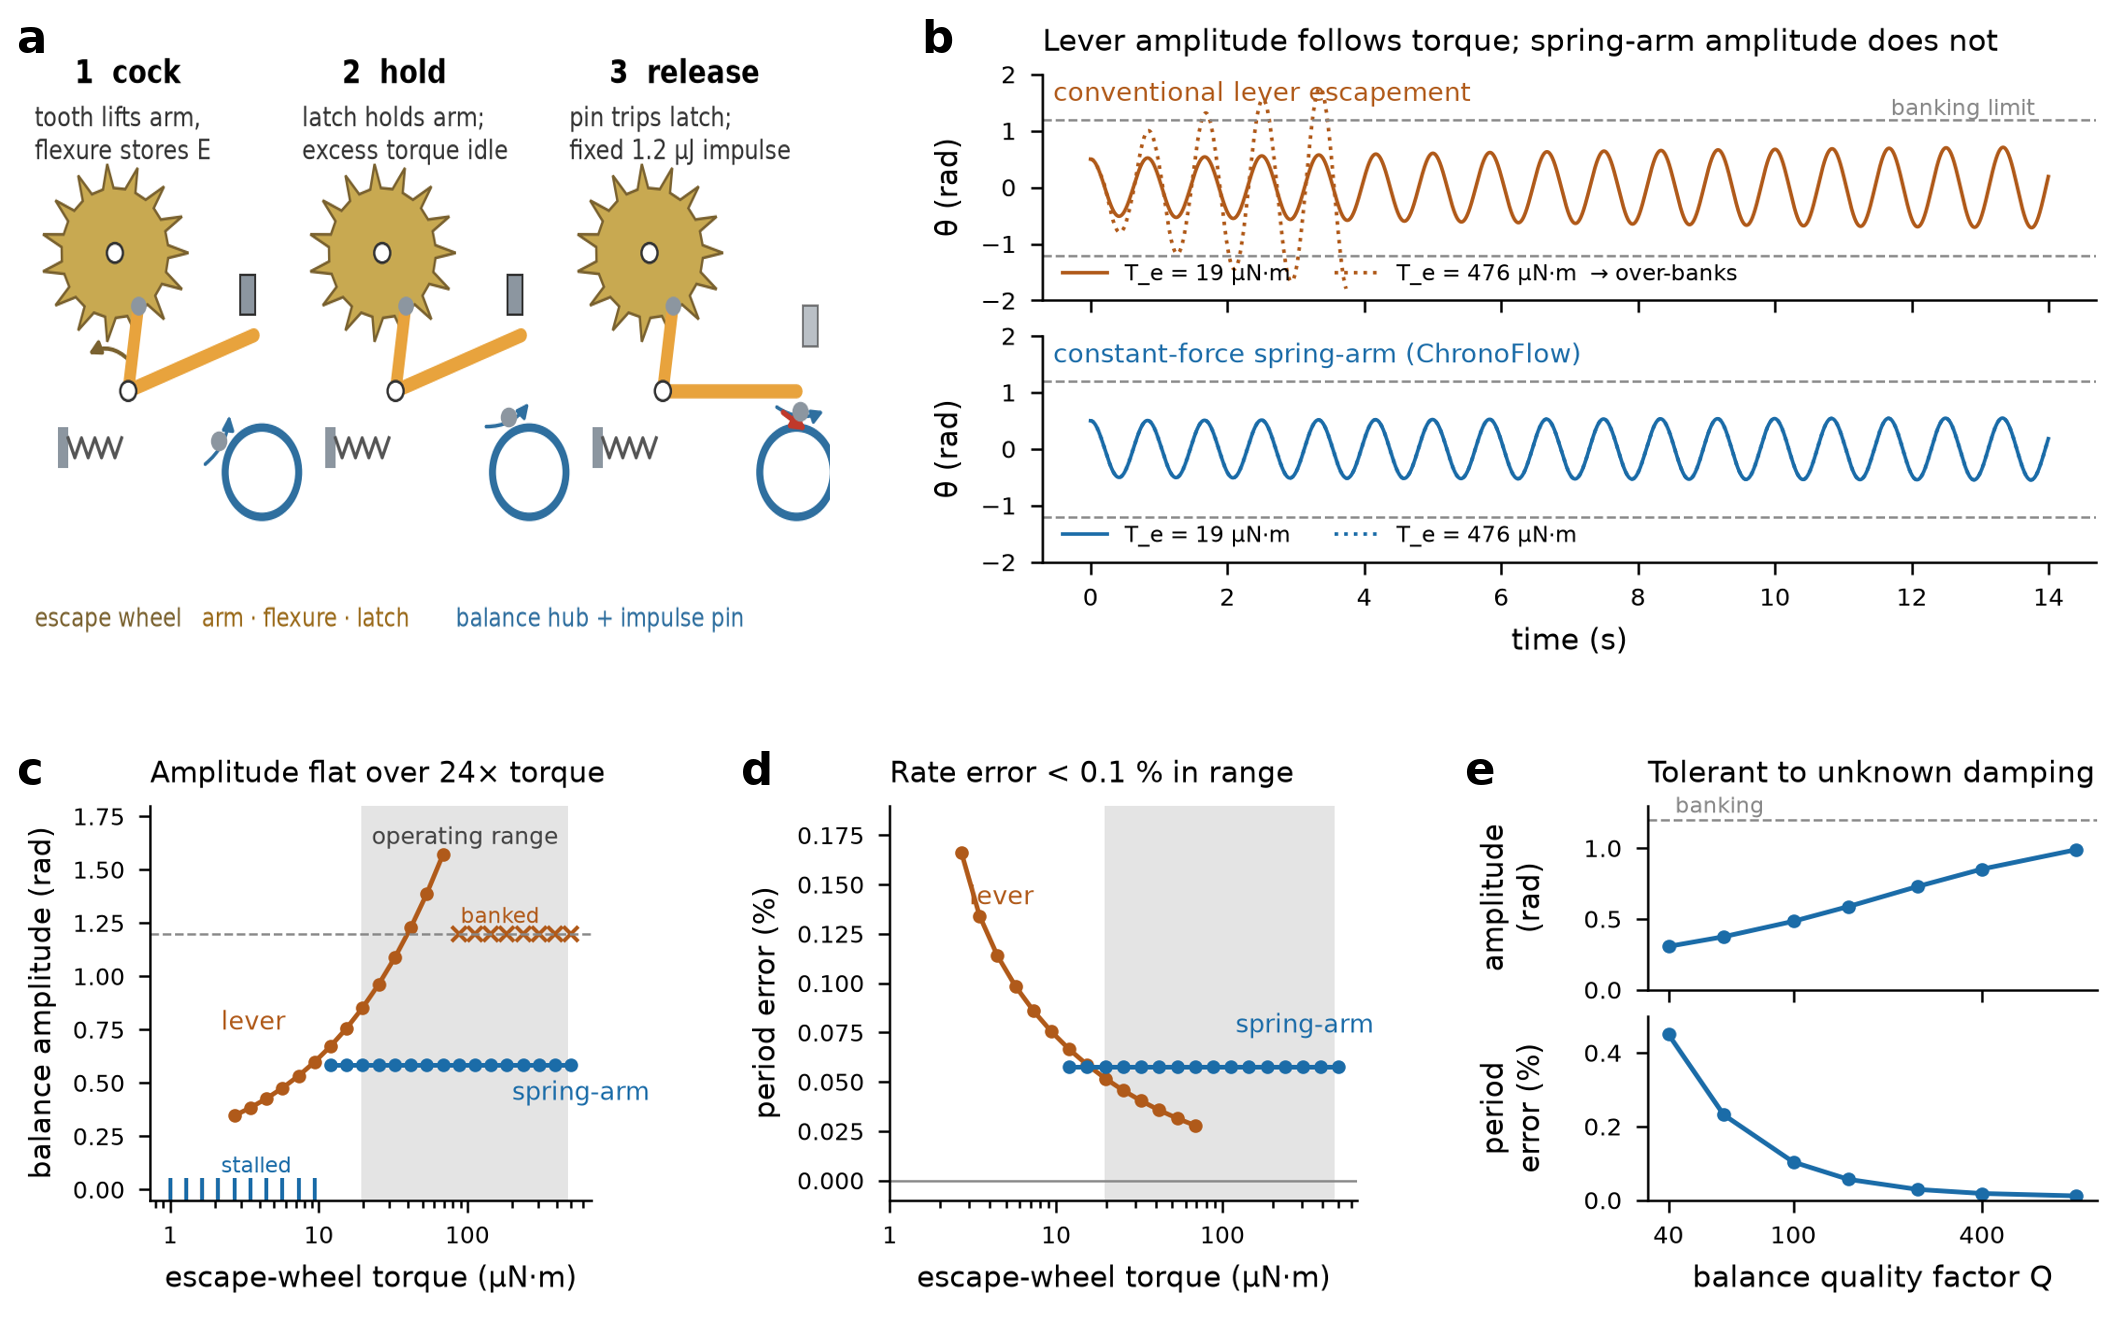
\includegraphics[width=\textwidth]{fig2.png}
\caption{\textbf{A constant-force spring-arm escapement keeps balance amplitude and rate independent of the $24\times$ variation in train torque that defeats a conventional lever escapement.} (a) Working principle: a wheel tooth cocks a spring-loaded impulse arm (1), a latch holds it while the wheel is locked (2), the balance pin trips the latch and receives a fixed impulse (3). (b) Simulated balance angle $\theta(t)$ for both escapements at the minimum and maximum operating torques (\SI{19}{} and \SI{476}{\micro\newton\metre}; RK4, $Q=150$); dashed lines mark the banking limit. (c) Steady amplitude and (d) period error relative to the free oscillator versus escape-wheel torque; shaded band: operating range. Ticks at zero mark torques below the spring-arm re-cock minimum. (e) Spring-arm amplitude and period error versus the balance quality factor $Q$.}
\label{fig:escapement}
\end{figure}

\begin{figure}[t]
\centering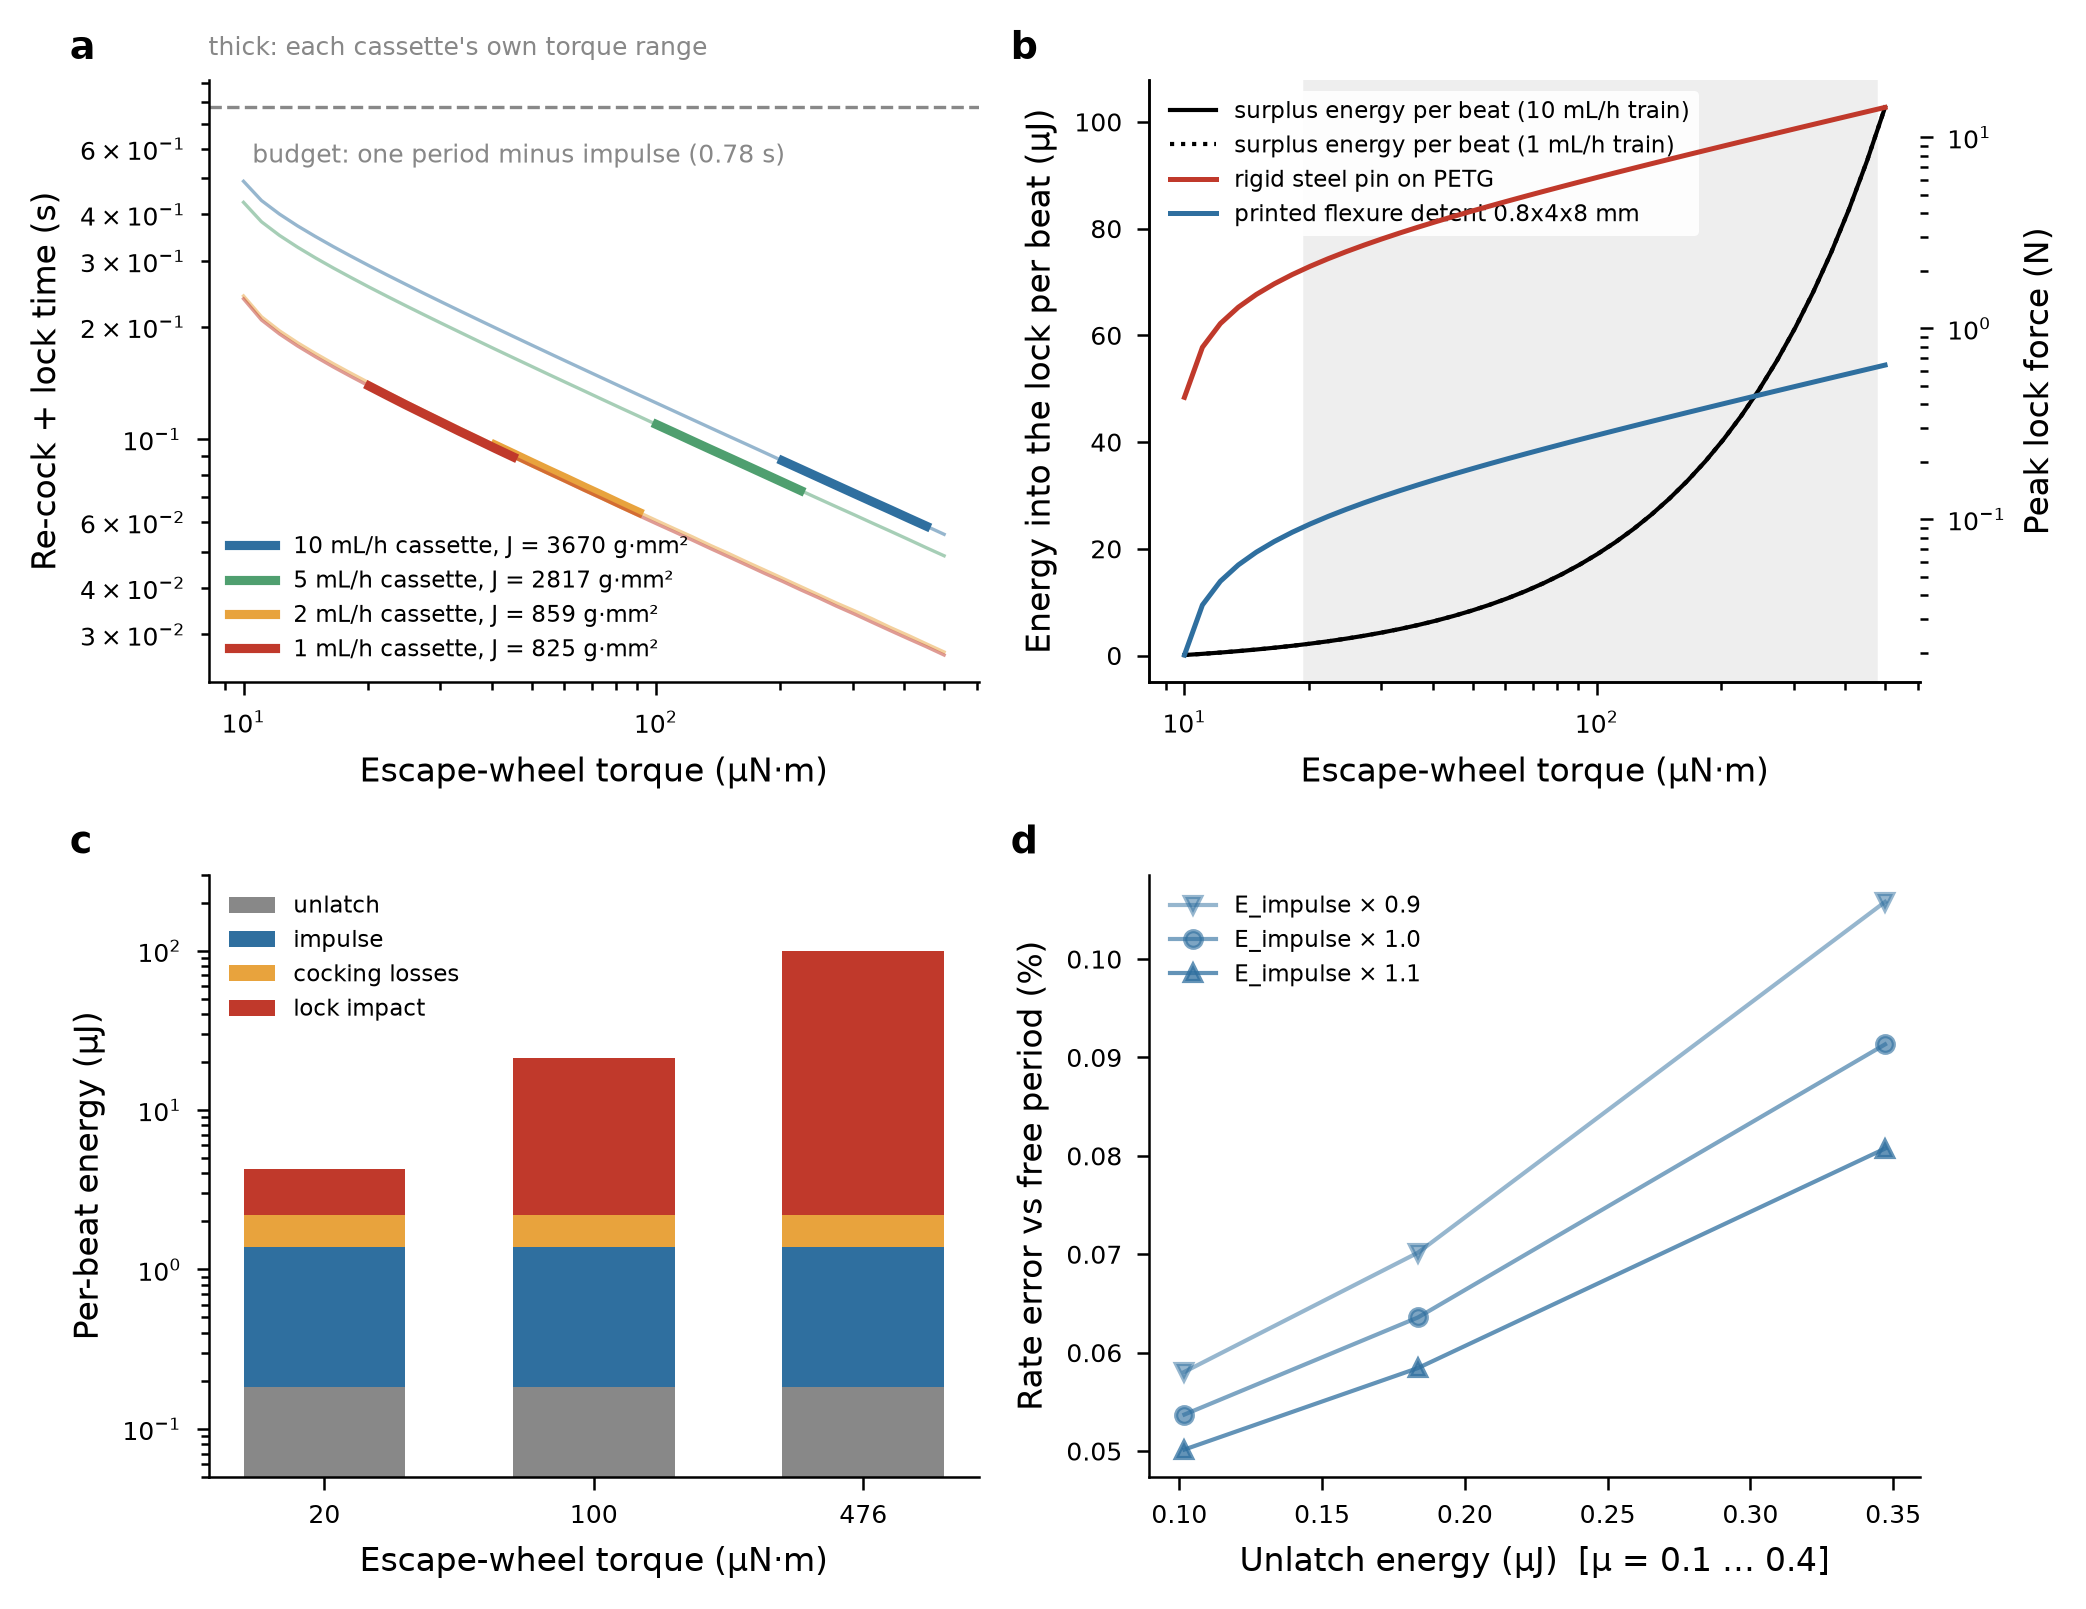
\includegraphics[width=\textwidth]{fig7.png}
\caption{\textbf{Mechanism-level analysis of the spring-arm escapement over the $24\times$ torque range.} (a) Time for the escape wheel to run half a pitch, re-cock the arm and lock, against the one-period budget; thick segments mark each cassette's own torque range, $J_{\mathrm{eff}}$ is the wheel plus reflected cassette inertia. (b) Surplus energy per beat arriving at the detent and the resulting peak lock force for a rigid steel-pin-on-PETG stop and for the \SI{2000}{\newton\per\metre} flexure detent. (c) Per-beat energy ledger at the minimum, a mid-range and the maximum torque. (d) Period error from the beat-level simulation for impulse energy $\pm\SI{10}{\percent}$ and unlatch work spanning $\mu = 0.1$--0.4.}
\label{fig:arm}
\end{figure}

\subsection{Taut-band balance}
The oscillator (Fig.~\ref{fig:oscillator}a) is a printed PETG ring (\SI{62}{\milli\metre} outer diameter, \SI{7.4}{\gram}, $I = \SI{5.2e-6}{\kilo\gram\metre\squared}$) clamped at the midpoint of a \SI{2}{\milli\metre}-wide spring-steel ribbon cut from a \SI{0.0015}{in} ($t = \SI{38.1}{\micro\metre}$) feeler-gauge blade, held at both ends and pre-tensioned to $T_0 = \SI{1}{\newton}$ by a steel coil spring. Each \SI{22}{\milli\metre} half-band is a torsion spring~\cite{timoshenko} of stiffness
\begin{equation}
k_{\mathrm{half}} = \frac{G J}{L_h} + \frac{T\,w^2}{12\,L_h}, \qquad J = \tfrac{1}{3} w t^3 \left(1 - 0.63\,\tfrac{t}{w}\right),
\end{equation}
giving $k = \SI{2.95e-4}{\newton\metre\per\radian}$ and $f_0 = \SI{1.20}{\hertz}$. Because $k \propto t^3$, the ribbon thickness is the dominant uncertainty: feeler stock is held to about \SI{\pm 2.5}{\micro\metre}, which alone would move $f_0$ by \SI{\pm 9}{\percent}, far beyond any trim-weight range (an earlier revision modelled a \SI{40}{\micro\metre} ribbon, \SI{6}{\percent} off the true stock). Regulation is therefore two-stage. Both end clamps are adjustable (Fig.~\ref{fig:cad}e): the upper clamp block is screwed through two M3 slots in a steel hanger plate bolted through the deck, and the lower clamp slides on guide pins in matching slots of a bracket that also carries the screwed spring-seat block of the tensioner, so the two are moved symmetrically and each half-band length $L_h$ can be set between 18 and \SI{26.5}{\milli\metre} while the hub stays centred; with $k = k_{\mathrm{half}}(L_{\mathrm{up}}) + k_{\mathrm{half}}(L_{\mathrm{low}})$ evaluated with each half's actual length, symmetric adjustment to 18.4--\SI{26.1}{\milli\metre} re-centres $f_0$ for any ribbon between 35.6 and \SI{40.6}{\micro\metre} (coarse, set once per ribbon). Adjusting one clamp alone would halve the sensitivity (\SI{1.1}{\percent} per mm against \SI{2.2}{\percent}) and the same slot would then cover only 36.6--\SI{39.4}{\micro\metre}, so one-sided adjustment is not sufficient; four M3 brass nuts in radial slots (23--\SI{29}{\milli\metre}) then regulate the frequency by $-2.4$ to \SI{+3.1}{\percent} (Fig.~\ref{fig:oscillator}b), exactly as a clock is regulated, with a nominal set point of \SI{26.4}{\milli\metre}.

Gravity enters only through the tension term: with the band vertical, the fixed-clamp half-band carries $T_0 \pm m g$ while the tensioner fixes the other at $T_0$. Because the tension term is \SI{10}{\percent} of $k$ and $mg \ll T_0$, the frequency shifts by only \SI{\pm 0.19}{\percent} between the upright and inverted positions (Fig.~\ref{fig:oscillator}c). An alternative two-leaf cross-spring flexure pivot~\cite{haringx}, analysed with an Euler--Bernoulli beam-column finite-element model including geometric stiffness, changed rotational stiffness by \SI{17}{\percent} under the same balance weight (the governing scale is $EI/L^2 \approx \SI{0.1}{\newton}$, not the Euler load) and was rejected. Peak shear stress at the \SI{1.2}{\radian} banking limit is \SI{166}{\mega\pascal} against a conservative fully-reversed fatigue limit of \SI{350}{\mega\pascal} (Fig.~\ref{fig:oscillator}d), and the temperature coefficient, combining the shear-modulus drift of steel with the thermal expansion of the ring, is $-1.8\times10^{-4}\,\mathrm{K}^{-1}$ (Fig.~\ref{fig:oscillator}e).

\begin{figure}[t]
\centering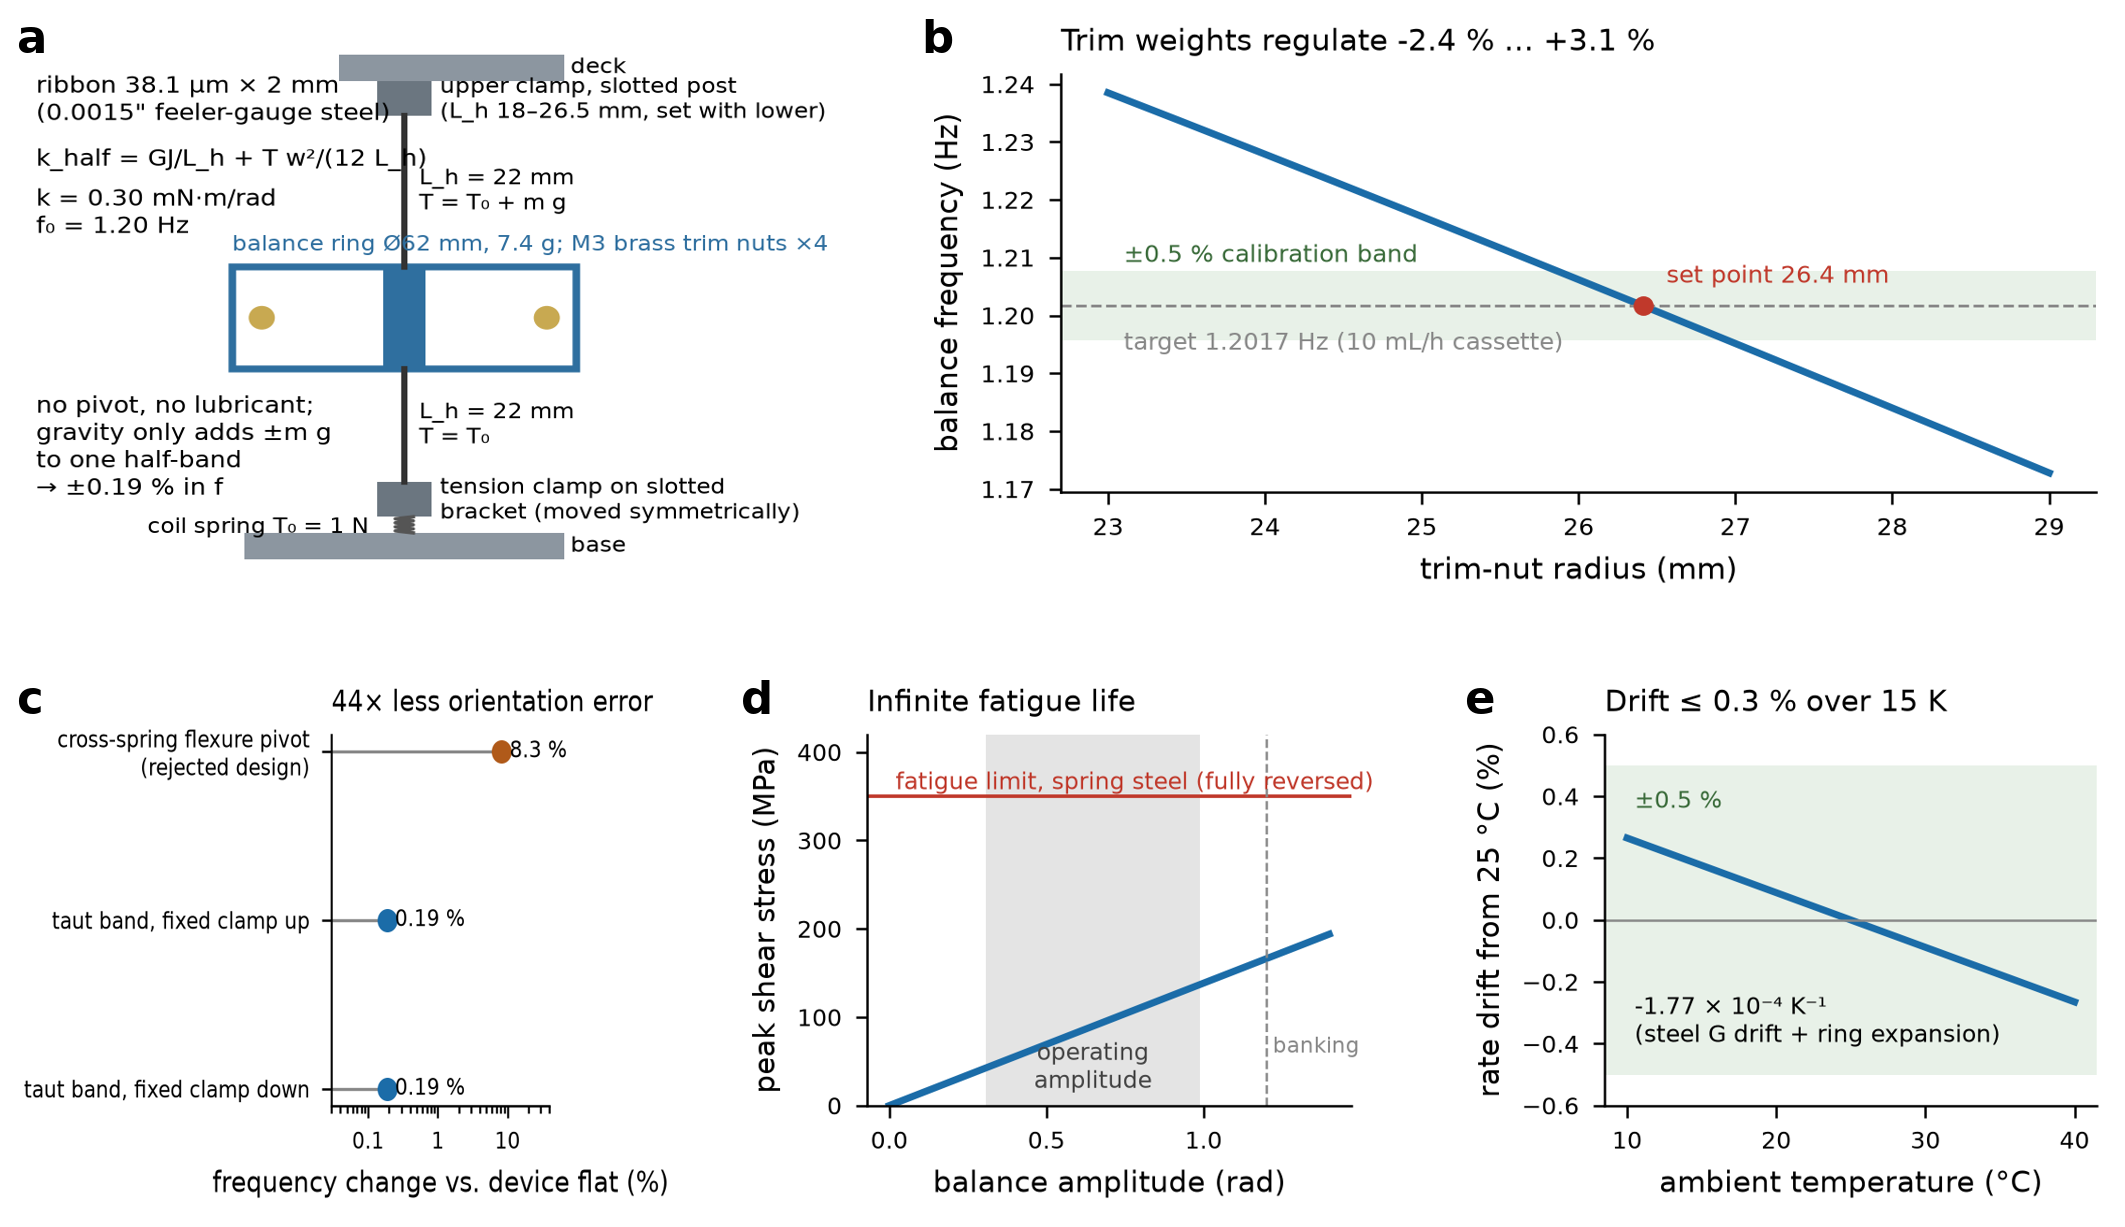
\includegraphics[width=\textwidth]{fig3.png}
\caption{\textbf{A taut-band suspension gives a friction-free \SI{1.2}{\hertz} balance whose rate is insensitive to orientation, temperature and fatigue.} (a) Construction: feeler-gauge ribbon clamped to the deck and to a spring-loaded tension clamp, balance ring clamped at mid-span. (b) Balance frequency versus radial position of the four trim nuts; the dashed line is the target for the unity cassette and the band is \SI{\pm 0.5}{\percent}. (c) Frequency change between the band-horizontal and band-vertical positions for the taut band, compared with the computed first-order change of a \SI{0.05}{\milli\metre} cross-spring flexure pivot under the same balance weight. (d) Peak ribbon shear stress versus amplitude; shaded band: amplitudes reached for $Q = 40$--800. (e) Rate drift versus ambient temperature.}
\label{fig:oscillator}
\end{figure}

\subsection{Rate cassettes, safety functions and structure}
A plug-in cassette carries two gear pairs with constant tooth sums ($z_1+z_2 = z_3+z_4 = 66$, \SI{33}{\milli\metre} centres): $(33,33,33,33)$, $(44,22,33,33)$, $(33,33,55,11)$ and $(44,22,55,11)$ give speed-up ratios of 1, 2, 5 and 10 and hence 10, 5, 2 and \SI{1}{\milli\litre\per\hour} on a \SI{20}{\milli\litre} BD syringe; other syringe sizes scale with bore area (Fig.~\ref{fig:system}a). The cassette is a visible, colour-coded object, so the set rate can be confirmed at a glance and cannot drift. Because the carriage speed is set by the cassette alone, the escape-wheel torque depends only on the cassette and on the excess force $F_{\mathrm{spring}} - F_{\mathrm{plunger}}$; the operating map was therefore evaluated over every syringe size, cassette and back-pressure from zero to the trip (80 cells). The torque exceeds the re-cock minimum of \SI{9.5}{\micro\newton\metre} by at least $2.0\times$ in every cell, the worst being the \SI{60}{\milli\litre} syringe on the \SI{1}{\milli\litre\per\hour} cassette at its \SI{300}{mmHg} trip (Fig.~\ref{fig:system}b). This map is what forced the drive spring from the \SI{30}{\newton} of the first revision to \SI{44.5}{\newton}: at \SI{30}{\newton} the \SI{60}{\milli\litre} trip left only \SI{3.1}{\newton} excess, \SI{3.4}{\micro\newton\metre} at the slowest cassette, and the escapement would have stalled before the occlusion flag was raised (two cells stalled, four below $1.7\times$). The per-beat volume is \SIrange{0.12}{1.16}{\micro\litre} (Fig.~\ref{fig:system}c).

Three safety functions are mechanical. (i) The occlusion trip (Fig.~\ref{fig:trip}; CAD in Fig.~\ref{fig:cad}c--d) is snap-acting. The pusher head rides on a \SI{8}{\milli\metre} steel stem backed by a \SI{3}{\newton\per\milli\metre} compression spring whose preload is set by a spacer keyed to each syringe cradle insert, so the setting follows the syringe size automatically. When the plunger reaction exceeds the preload the stem retracts; a trip pin on its end collar stands \SI{0.15}{\milli\metre} behind the tail of a sear, a printed plate on a vertical pivot whose hook lip overlaps a collar on a separate flag rod by \SI{0.9}{\milli\metre}. The sear's lever ratio (hook arm 9, tail arm \SI{2}{\milli\metre}) is 4.5, so the lip clears the collar after a further \SI{0.20}{\milli\metre}: the \emph{sensing travel} is $0.15 + 0.9/4.5 = \SI{0.35}{\milli\metre}$, and it is a geometric property of the modelled parts rather than an assumption. The flag rod, driven by its own \SI{2}{\newton} spring, then rises \SI{6}{\milli\metre} and does three things: it exposes the red flag; its lift collar frees a torsion-sprung rocker on the carriage top whose short end drives a \SI{2}{\milli\metre} steel capture pin \SI{2.2}{\milli\metre} down into a slot in the stem top; and its head lifts a frame-mounted rail that runs the length of the carriage travel on two parallel-motion cranks, so the rail translates by the same \SI{6}{\milli\metre} wherever the carriage is. A drop rod from the rail passes through the deck and raises a two-pin fork (pins at \SI{80}{} and \SI{100}{\degree}, $r = \SI{18}{\milli\metre}$) around a balance spoke, confining the balance to \SI{\pm 0.05}{\radian}---below the \SI{6}{\degree} unlock angle---so the escapement cannot unlock, ticking stops and pressure cannot rise further. Defining the trip at \SI{0.35}{\milli\metre} rather than at a full \SI{3}{\milli\metre} of stem travel matters: over \SI{3}{\milli\metre} the spring force would rise by \SI{9}{\newton} (\SI{+235}{mmHg} on a \SI{20}{\milli\litre} syringe, and enough to take the \SI{60}{\milli\litre} case below the re-cock minimum before the flag appeared); over \SI{0.35}{\milli\metre} it rises by \SI{1.05}{\newton}, and the spacer preload is set \SI{1.05}{\newton} below the intended trip force so that the sear releases at $300\,\mathrm{mmHg}\times A + F_{\mathrm{friction}}$: trip forces 6.1, 8.6, 14.5, 18.3 and \SI{26.9}{\newton} from spacer preloads of 5.0, 7.6, 13.4, 17.2 and \SI{25.8}{\newton} (1.7--\SI{8.6}{\milli\metre}) for the 5, 10, 20, 30 and \SI{60}{\milli\litre} syringes. The operating-map margins above are therefore unchanged by the trip. The slot's forward wall is cut \SI{0.35}{\milli\metre} short of the pin, so that after the sensing travel it is flush with the pin and the \SI{0.35}{\milli\metre} of spring compression stored at the trip (0.04--\SI{0.20}{\milli\litre} of syringe volume, 60~mL largest) cannot advance the plunger when the blockage clears; this is checked on the solids rather than asserted: posing the tripped assembly with the stem advanced by 0.1 and \SI{0.2}{\milli\metre} produces pin--stem interference (0.08 and \SI{0.24}{\milli\metre\cubed}), while the armed and tripped poses are interference-free, and rotating the balance by \SI{\pm 0.04}{\radian} inside the raised fork is free but \SI{\pm 0.08}{\radian} is blocked. The mechanism's own release bolus is thus zero by construction, and what remains is the elastic volume stored in the line and syringe at \SI{300}{mmHg}, which the protocol measures against the \SI{0.2}{\milli\litre} target. Reset is only through the LOAD/RUN lever, which re-cocks the flag rod (re-engaging the sear and lifting the rocker and capture pin) and lowers the rail. A force trip senses friction as well as pressure, so the pressure at which it fires carries the friction uncertainty: for \SI{\pm 1.5}{\newton} of plunger glide-force variation (lot, speed, dwell) the \SI{300}{mmHg} setting fires between 280 and \SI{320}{mmHg} on the \SI{60}{\milli\litre} syringe but between 202 and \SI{398}{mmHg} on the \SI{5}{\milli\litre} syringe, whose bore is five times smaller. These bands are the disclosed occlusion-alarm range; tightening them for the small syringes requires measuring glide force per syringe lot and shimming the spacer, which the validation protocol includes. (ii) The LOAD/RUN lever opens the syringe flange latch and lifts the rack-pinion click together, so the carriage can only be moved by hand when the syringe is unlatched and a fast-forwarded pusher slides the whole syringe rather than expelling fluid. (iii) The balance beats behind a window at \SI{1.2}{\hertz}; silence means stopped.

The most heavily loaded teeth are the rack and 12-tooth pinion: Lewis bending stress~\cite{lewis} at \SI{44.5}{\newton} on an \SI{8}{\milli\metre} face is \SI{22.7}{\mega\pascal} against about \SI{50}{\mega\pascal} PETG yield (safety factor 2.2; widening the stage-1 face to \SI{10}{\milli\metre} would restore 2.75). Torque falls $5\times$ per stage (267, 49, 9.0, \SI{1.7}{\milli\newton\metre}), so the remaining printed gears are lightly loaded; shafts are \SI{3}{\milli\metre} steel pins in printed bores.

\begin{figure}[t]
\centering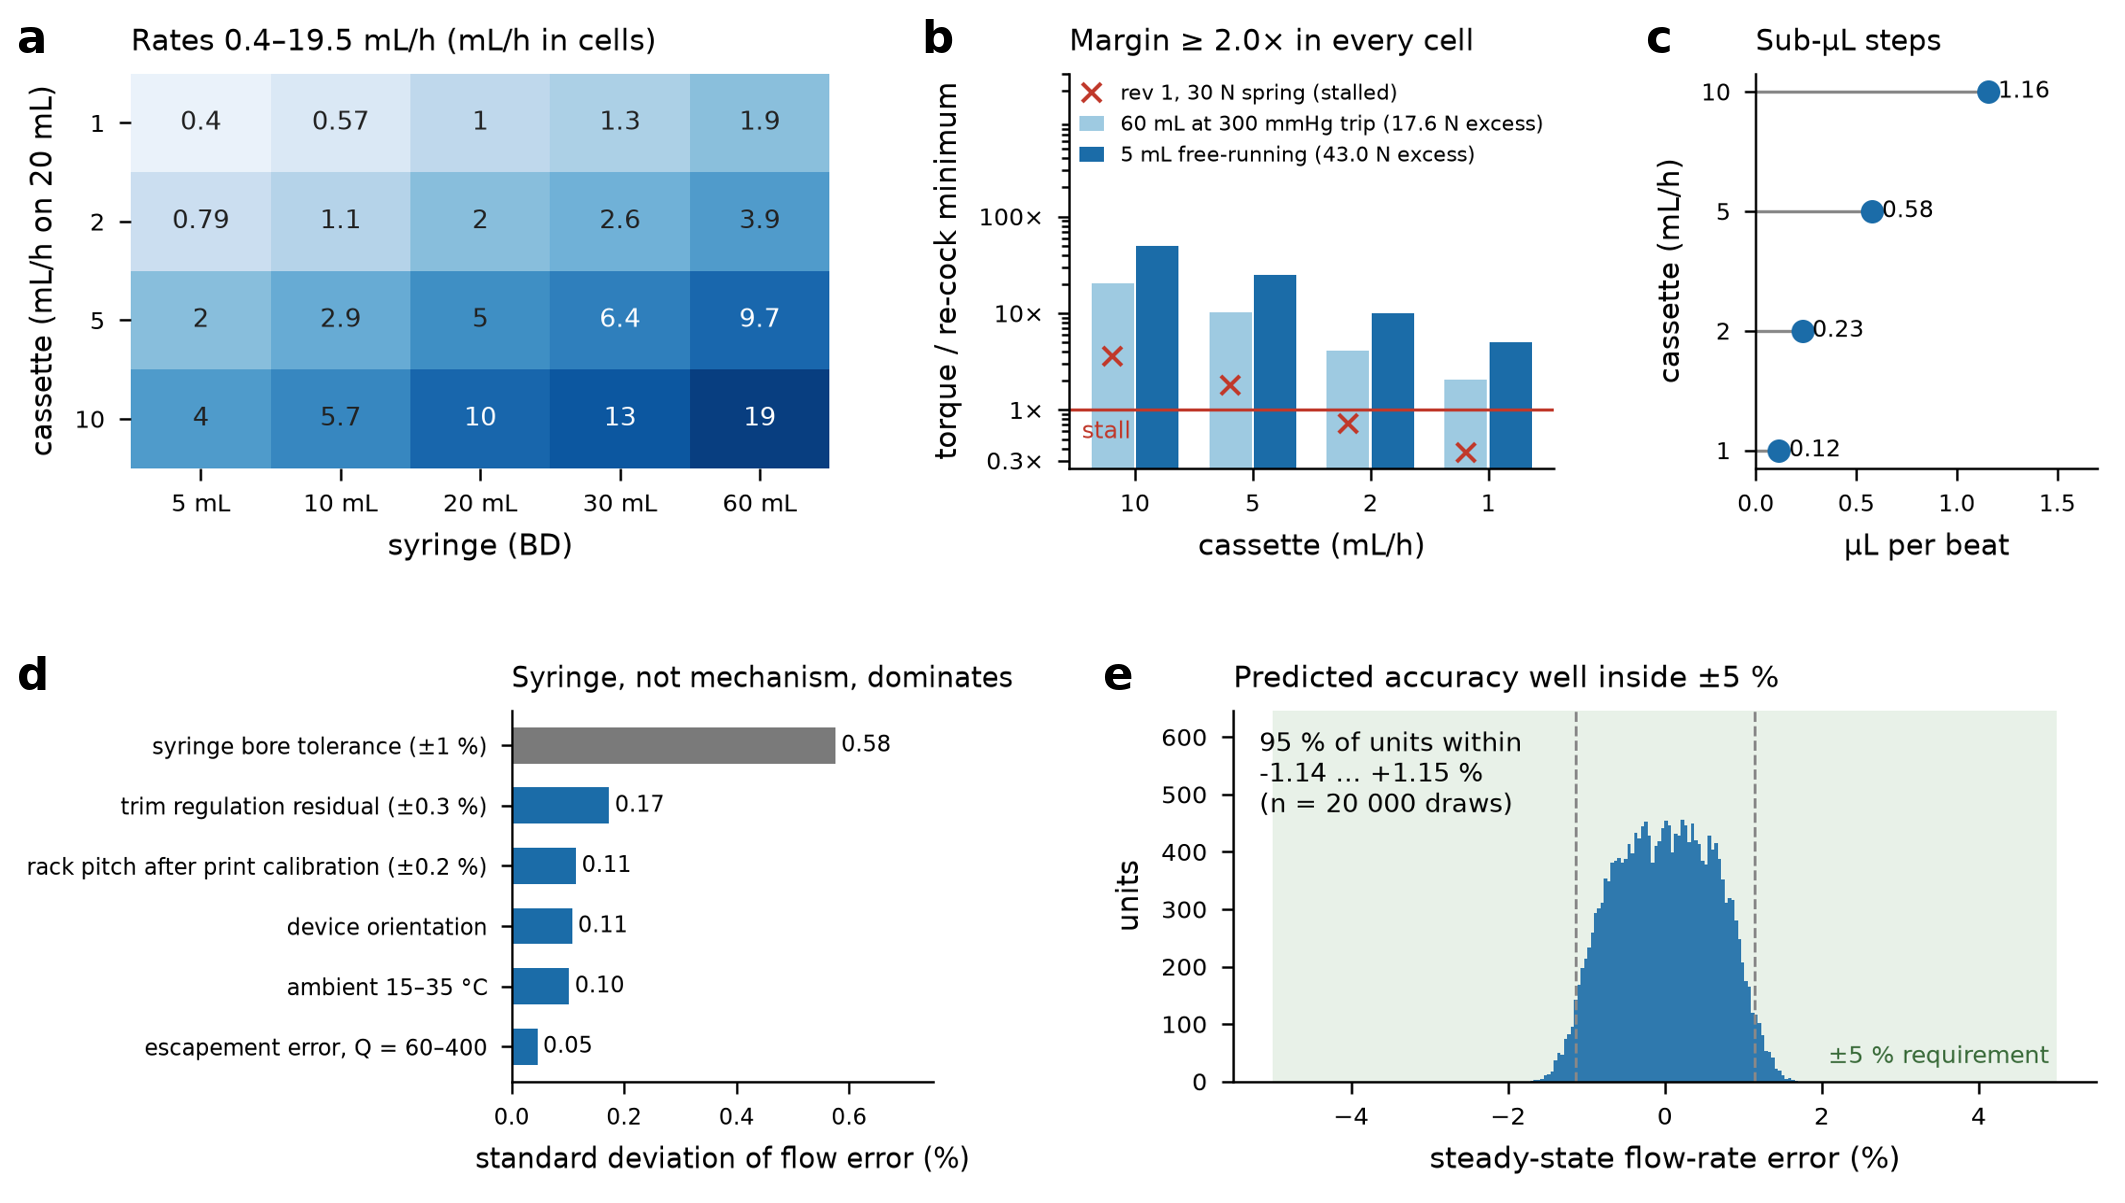
\includegraphics[width=\textwidth]{fig4.png}
\caption{\textbf{Four plug-in cassettes cover neonatal rates with torque margin and sub-microlitre resolution; the predicted error is dominated by the syringe, not the mechanism.} (a) Flow rate for each cassette and BD syringe size. (b) Escape-wheel torque relative to the arm re-cock minimum at the two extremes of the syringe $\times$ cassette $\times$ pressure map (\SI{60}{\milli\litre} syringe at its \SI{300}{mmHg} trip; \SI{5}{\milli\litre} syringe free-running); crosses show the first revision's \SI{30}{\newton} spring, which stalled. (c) Volume delivered per beat. (d) Standard deviation of flow error contributed by each Monte-Carlo input. (e) Distribution of steady-state flow error over 20\,000 draws; dashed lines mark the central \SI{95}{\percent}.}
\label{fig:system}
\end{figure}

\begin{figure}[t]
\centering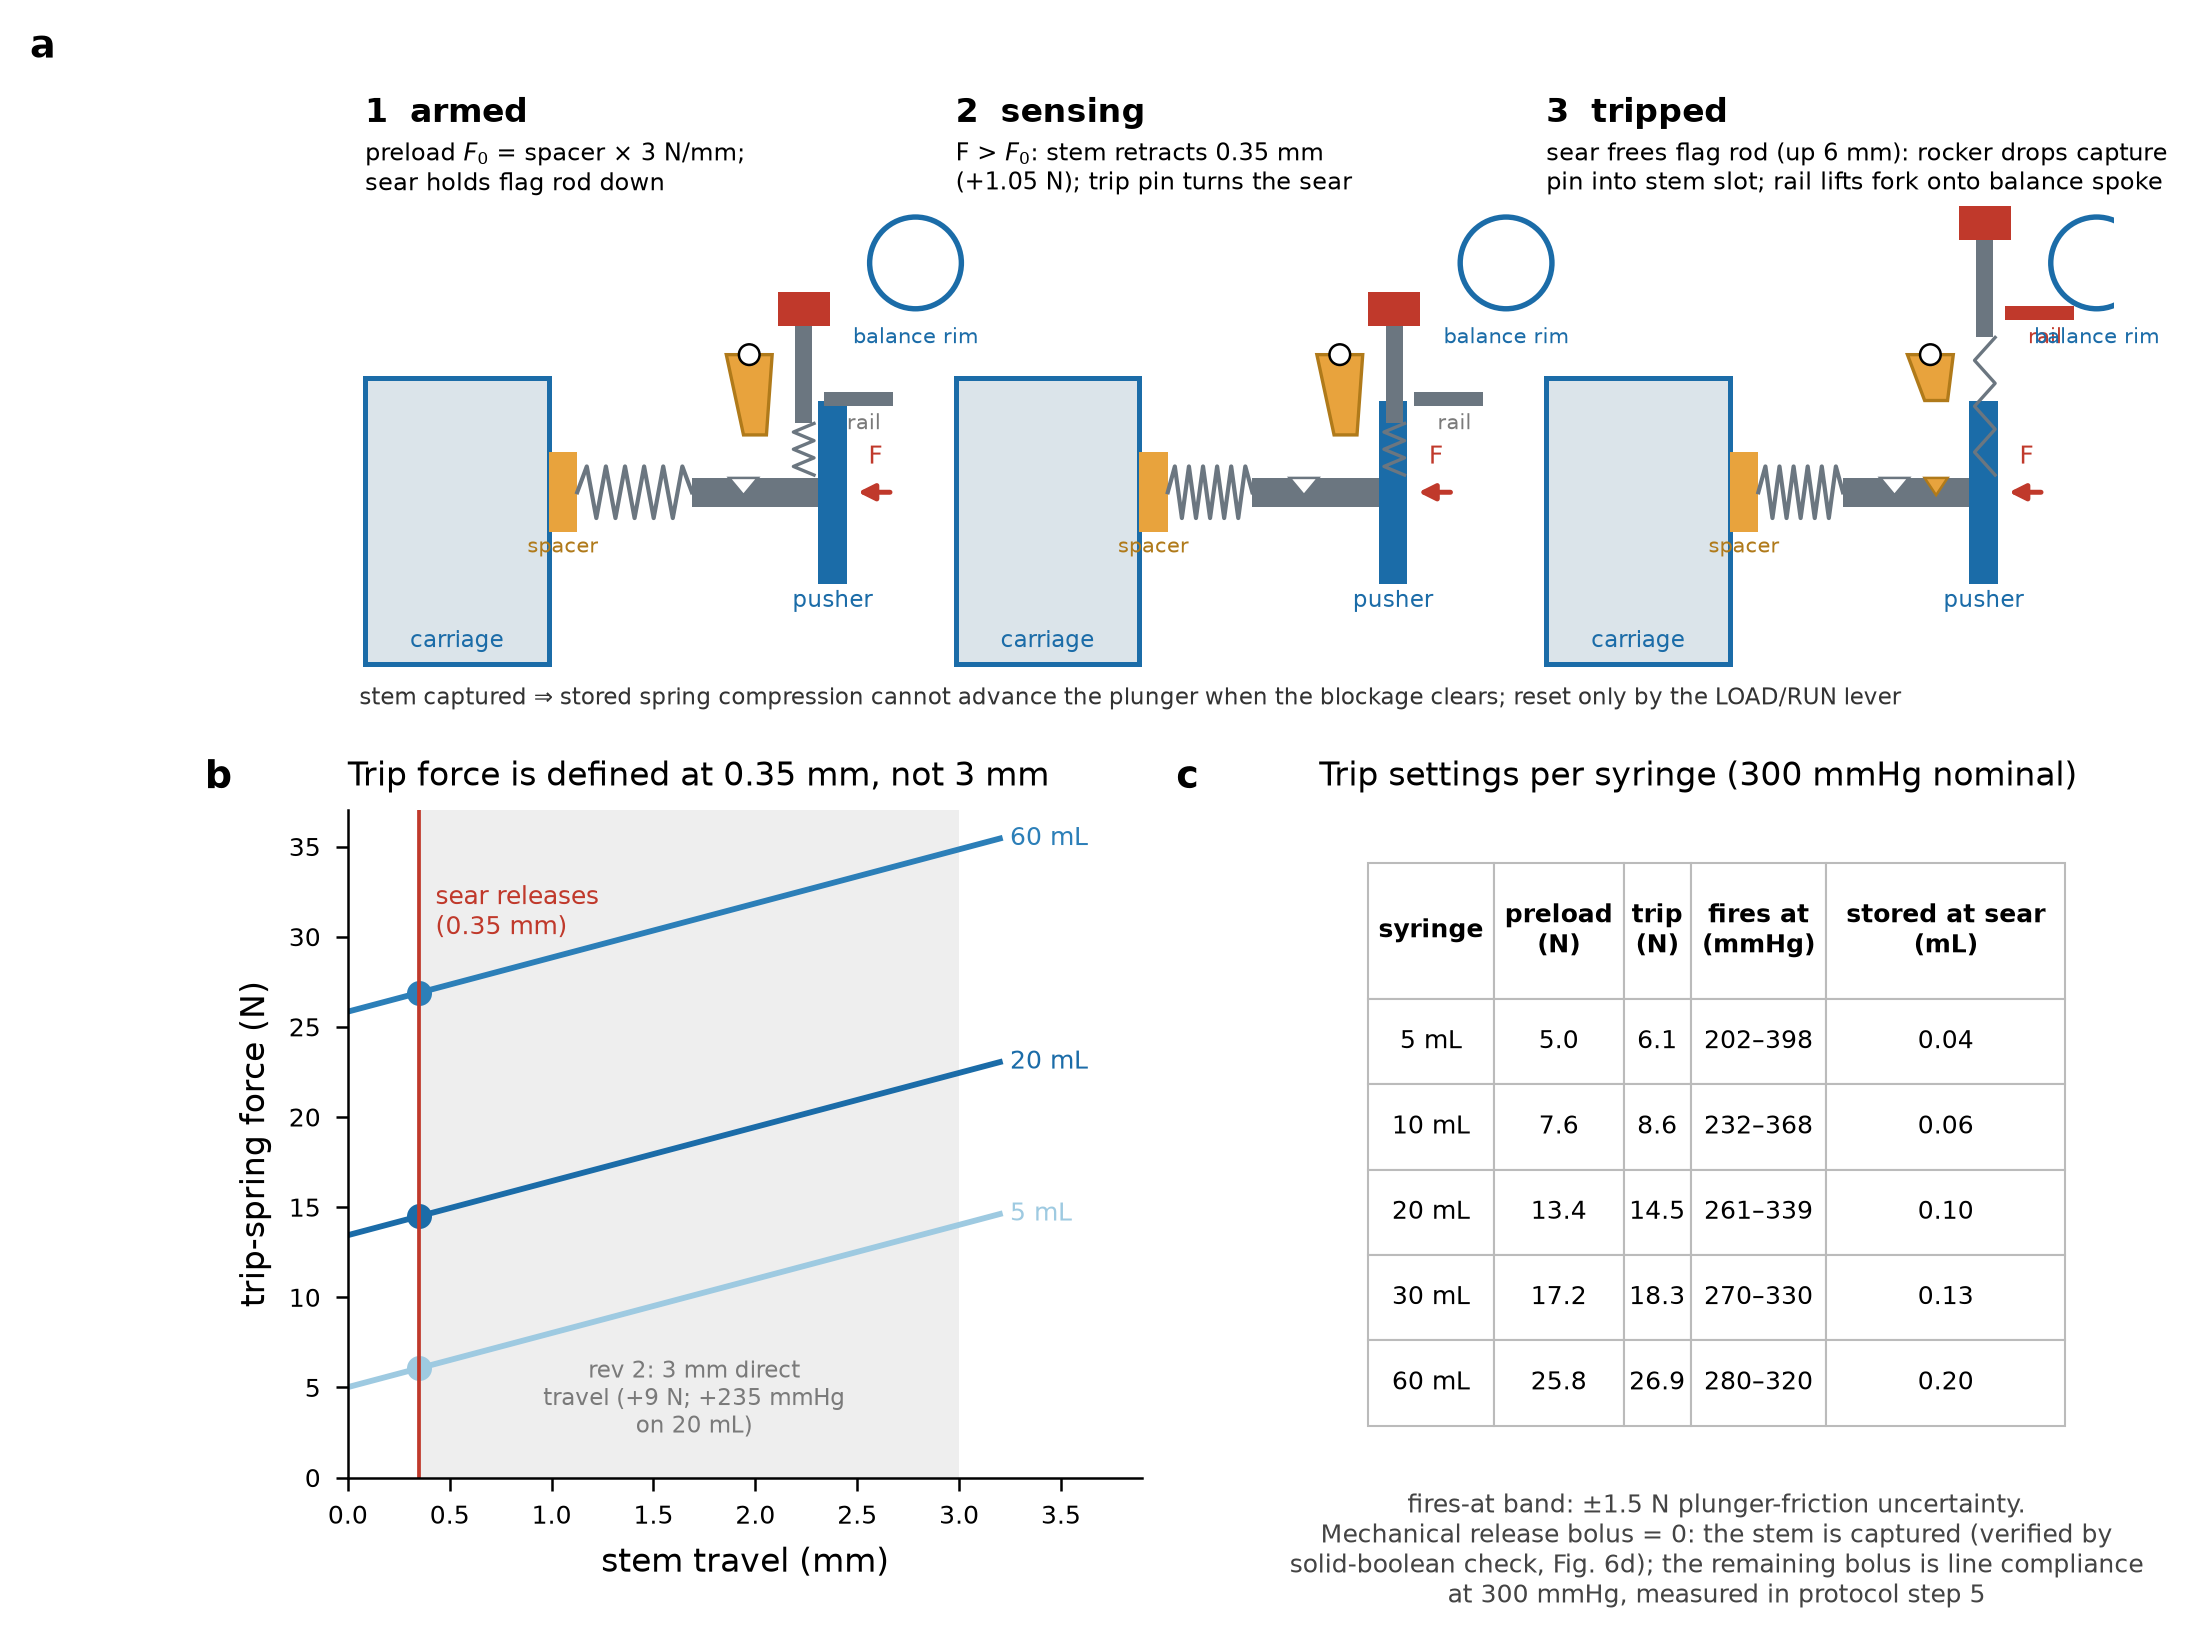
\includegraphics[width=\textwidth]{fig6.png}
\caption{\textbf{Snap-action occlusion trip: the trip force is defined by a \SI{0.35}{\milli\metre} sensing travel set by the sear geometry, and the stem is captured so stored spring compression cannot become a bolus.} (a) Armed, sensing and tripped states (schematic; the modelled parts are in Fig.~\ref{fig:cad}c--d): spacer-set preload, \SI{0.35}{\milli\metre} stem retraction turns the sear, \SI{6}{\milli\metre} flag-rod release drops the capture pin into the stem slot and lifts the rail and balance fork. (b) Trip-spring force versus stem travel for three syringe sizes; the sear releases at \SI{0.35}{\milli\metre} (+\SI{1.05}{\newton}, pre-compensated in the spacer); the grey band is the \SI{3}{\milli\metre} direct-travel design of the previous revision. (c) Per-syringe spacer preload, trip force, firing band for \SI{\pm 1.5}{\newton} plunger-friction uncertainty, and the displacement stored at the sear if the stem were not captured.}
\label{fig:trip}
\end{figure}


\section{Methods}\label{sec:methods}
\paragraph{Parametric design.} All dimensions, tooth counts and oscillator parameters live in one module (\texttt{design\_params.py}); the CAD (\texttt{cad\_model.py}, CadQuery~2.8) derives shaft positions from gear centre distances, phases every mesh so that a wheel tooth faces a pinion gap, and exports STEP, glTF and per-part STL. The gear train is posed with the carriage: every gear is rotated by the rack displacement through the seven meshes (the displacement being trimmed by $<\SI{0.03}{\milli\metre}$ so that the escape wheel sits at a locked tooth). A pairwise interference check (bounding-box prefilter, OpenCascade Boolean common) is run over all 4\,095 part pairs in twelve poses---carriage at full, half and empty syringe, armed and tripped, balance at rest and at \SI{\pm 0.6}{\radian}. Overlaps are compared against an explicit list of eighteen named part pairs, each with a physical reason and a volume cap (press-fit pins, threaded screws, the drawn \SI{0.1}{\milli\metre} penetration of a locked tooth, the tooth-tip overlap of the unshifted 12-tooth pinions, $\leq\SI{0.7}{\milli\metre\cubed}$); anything else above \SI{0.05}{\milli\metre\cubed} is a fault. The earlier keyword whitelist (any pair containing ``pin'', ``shaft'' or ``axle'') and single pose were replaced in this revision; the multi-pose check found and fixed three real collisions (rack against the cradle at the empty-syringe position, the trip rail's rear post against the carriage at full travel, and the capture-pin rocker against its boss in the tripped pose) and the last run reports zero faults in all twelve poses (\texttt{results/interference\_report.json}). All 91 exported STL meshes are watertight (the carriage rack previously ran a partial last tooth past its end and produced a self-intersecting profile).

\paragraph{Escapement dynamics.} The balance obeys $I\ddot\theta = -k\theta - c\dot\theta + \tau(\theta,\dot\theta)$ with $c = I\omega_0/Q$, integrated by fourth-order Runge--Kutta at $\Delta t = \SI{0.2}{\milli\second}$. For the lever model the per-beat wheel energy $T_e\pi/Z_e$ is split into an impulse fraction (0.70) applied over a \SI{30}{\degree} lift arc and an unlocking fraction (0.12) opposing motion over \SI{6}{\degree}. For the spring-arm model the impulse energy is fixed at $E_{\mathrm{imp}}$ over \SI{15}{\degree} starting \SI{3}{\degree} before equilibrium, with a fixed \SI{0.12}{\micro\joule} latch-tripping cost; the escapement stalls if $T_e < T_{\min}$. A reversal of the balance while the pin is inside the engagement window is treated as a fault. Period is measured over steady-state zero crossings. The mechanism-level model (\texttt{analysis\_arm\_mechanism.py}) integrates the wheel, $J_{\mathrm{eff}}\ddot\varphi = T_e - T_{\mathrm{cock}}(\varphi) - c\dot\varphi$, from the unlock to the lock over the free arc and a \SI{0.1}{\radian} cocking arc, with $J_{\mathrm{eff}}$ the wheel plus every upstream gear reflected by its speed ratio squared; lock forces use $F = \sqrt{2 E k_{\mathrm{stop}}}$ and Hertz line contact for a \SI{1}{\milli\metre} steel pin on PETG ($E^* = \SI{2.2}{\giga\pascal}$).

\paragraph{Oscillator.} Band stiffness follows Timoshenko's thin-strip torsion with the tension term; the cross-spring pivot comparison uses a 60-element Euler--Bernoulli beam-column model per leaf (elastic plus geometric stiffness), with the balance rotating rigidly about the crossing point and gravity resolved onto the two leaves.

\paragraph{Error budget.} 20\,000 Monte-Carlo draws combine uniform syringe bore tolerance (\SI{\pm 1}{\percent} area, ISO~7886-1 class~\cite{iso7886}), trim regulation residual (\SI{\pm 0.3}{\percent}), rack pitch after print-scale calibration (\SI{\pm 0.2}{\percent}), ambient temperature (15--\SI{35}{\celsius}), orientation (\SI{\pm 0.19}{\percent}) and the escapement error for $Q$ uniformly in 60--400 after calibration at the mean.

\paragraph{Comparators.} Flow-restriction pumps are modelled as $Q \propto (P_{\mathrm{drive}} - P_{\mathrm{back}})/\mu(T)$ with water viscosity from the Vogel equation~\cite{vogel} ($\mu = 0.02939\,\exp[507.88/(T-149.3)]$~\si{\milli\pascal\second}) and drive pressures of 300 and \SI{500}{mmHg}.

\section{Results}
\begin{table}[t]
\centering\small
\caption{Predicted performance of \ChronoFlow\ (BD \SI{20}{\milli\litre} syringe unless stated) and bill of materials.}
\label{tab:summary}
\begin{tabular}{@{}p{0.26\textwidth}p{0.70\textwidth}@{}}
\toprule
Quantity & Value \\
\midrule
Rates (cassettes 1/2/5/10) & 1, 2, 5, \SI{10}{\milli\litre\per\hour}; \SIrange{0.4}{19.5}{\milli\litre\per\hour} across 5--\SI{60}{\milli\litre} syringes \\
Resolution & \SIrange{0.12}{1.16}{\micro\litre} per beat, 2.4 beats\,s$^{-1}$ \\
Oscillator & \SI{1.2017}{\hertz}; coarse $L_h$ 18--\SI{26.5}{\milli\metre}, trim $-2.4$/\SI{+3.1}{\percent}; orientation \SI{\pm 0.19}{\percent}; $-1.8\times10^{-4}$\,K$^{-1}$ \\
Escapement & amplitude \SI{0.59}{\radian} ($Q=150$), period error \SI{0.06}{\percent} (0.05--\SI{0.11}{\percent} over $E_{\mathrm{imp}}\pm\SI{10}{\percent}$, $\mu$ 0.1--0.4); torque margin $\geq 2.0\times$ over 5 syringes $\times$ 4 cassettes $\times$ 0--\SI{300}{mmHg}; re-cock time $\leq\SI{0.14}{\second}$ vs \SI{0.77}{\second}; detent impact $\leq\SI{0.63}{\newton}$, \SI{19}{\mega\pascal} with flexure detent \\
Accuracy (Monte-Carlo, $n$ = 20\,000) & \SI{95}{\percent} of units within $-1.14$ to \SI{+1.15}{\percent}; 99th percentile $|{\rm error}|$ \SI{1.36}{\percent} \\
Restriction-pump comparator & \SI{+45}{\percent} at \SI{37}{\celsius}; \SI{-23}{\percent} at \SI{10}{\celsius}; \SI{-33}{\percent} at \SI{100}{mmHg} back-pressure \\
Occlusion trip & \SI{300}{mmHg} nominal; snap-action sear at \SI{0.35}{\milli\metre} sensing travel (from the sear geometry), spacer preload keyed to cradle insert (5.0--\SI{25.8}{\newton}, trip 6.1--\SI{26.9}{\newton}); fires at 280--320 (\SI{60}{\milli\litre}) to 202--\SI{398}{mmHg} (\SI{5}{\milli\litre}) for \SI{\pm 1.5}{\newton} friction; stem captured by a pin in a slot (solid-boolean verified), mechanical release bolus 0 \\
Energy & \SI{4.2}{\joule} stored per wind; \SI{0.37}{\joule} consumed in \SI{20}{\hour} \\
Structure & rack-pinion tooth stress \SI{22.7}{\mega\pascal} (SF 2.2); band stress \SI{166}{\mega\pascal} vs \SI{350}{\mega\pascal} limit \\
Parts, cost & 91 parts, $\approx$\SI{420}{\gram} PETG, BOM $\approx$\,\$40; zero interference faults in 12 poses; 91/91 STL meshes watertight \\
\bottomrule
\end{tabular}
\end{table}

Table~\ref{tab:summary} collects the predicted performance. Two results carry the design. First, the escapement study (Fig.~\ref{fig:escapement}) shows that the conventional lever escapement is unusable across the clinical range---its amplitude passes the banking limit at about \SI{40}{\micro\newton\metre}, below the mid-point of the operating band---whereas the spring-arm escapement holds \SI{0.59}{\radian} from the re-cock minimum upward with a period error of \SI{0.06}{\percent}. Second, the suspension study (Fig.~\ref{fig:oscillator}) shows that the taut band reduces orientation sensitivity by a factor of about forty relative to a cross-spring pivot of the same leaf stock, while keeping the ribbon stress at \SI{47}{\percent} of the fatigue limit at the banking amplitude. The system-level consequences (Fig.~\ref{fig:system}) are a rate set entirely by integers (tooth counts) and one calibrated frequency, a torque margin above the re-cock threshold at every rate, and a predicted accuracy distribution whose width is set mainly by the syringe bore tolerance that every syringe pump shares.

Against flow-restriction pumps the difference is categorical rather than incremental (Fig.~\ref{fig:overview}c--d): a restriction pump calibrated at \SI{20}{\celsius} over-delivers by \SI{45}{\percent} at body temperature and loses a third of its rate against \SI{100}{mmHg} of venous or catheter back-pressure, whereas \ChronoFlow\ drifts by less than \SI{0.4}{\percent} over 10--\SI{40}{\celsius} and is unaffected by back-pressure until it trips.

The CAD model (Fig.~\ref{fig:cad}) is complete at the part level: deck and bottom plates, pillars, rails, cradle with flange latch and barrel clamp, carriage with integrated rack, the pusher stem with keyed spacer, trip spring, sear, flag rod, rocker and capture pin, the trip rail with its cranks, drop rod and balance fork, spring drum, the four-stage train, cassette, escape wheel, two impulse arms with latch and the wheel detent, and the balance with band, slotted clamps and tensioner. The model is built in two states (armed and tripped) and the capture function is demonstrated on the solids (Fig.~\ref{fig:cad}c--d).

\begin{figure}[t]
\centering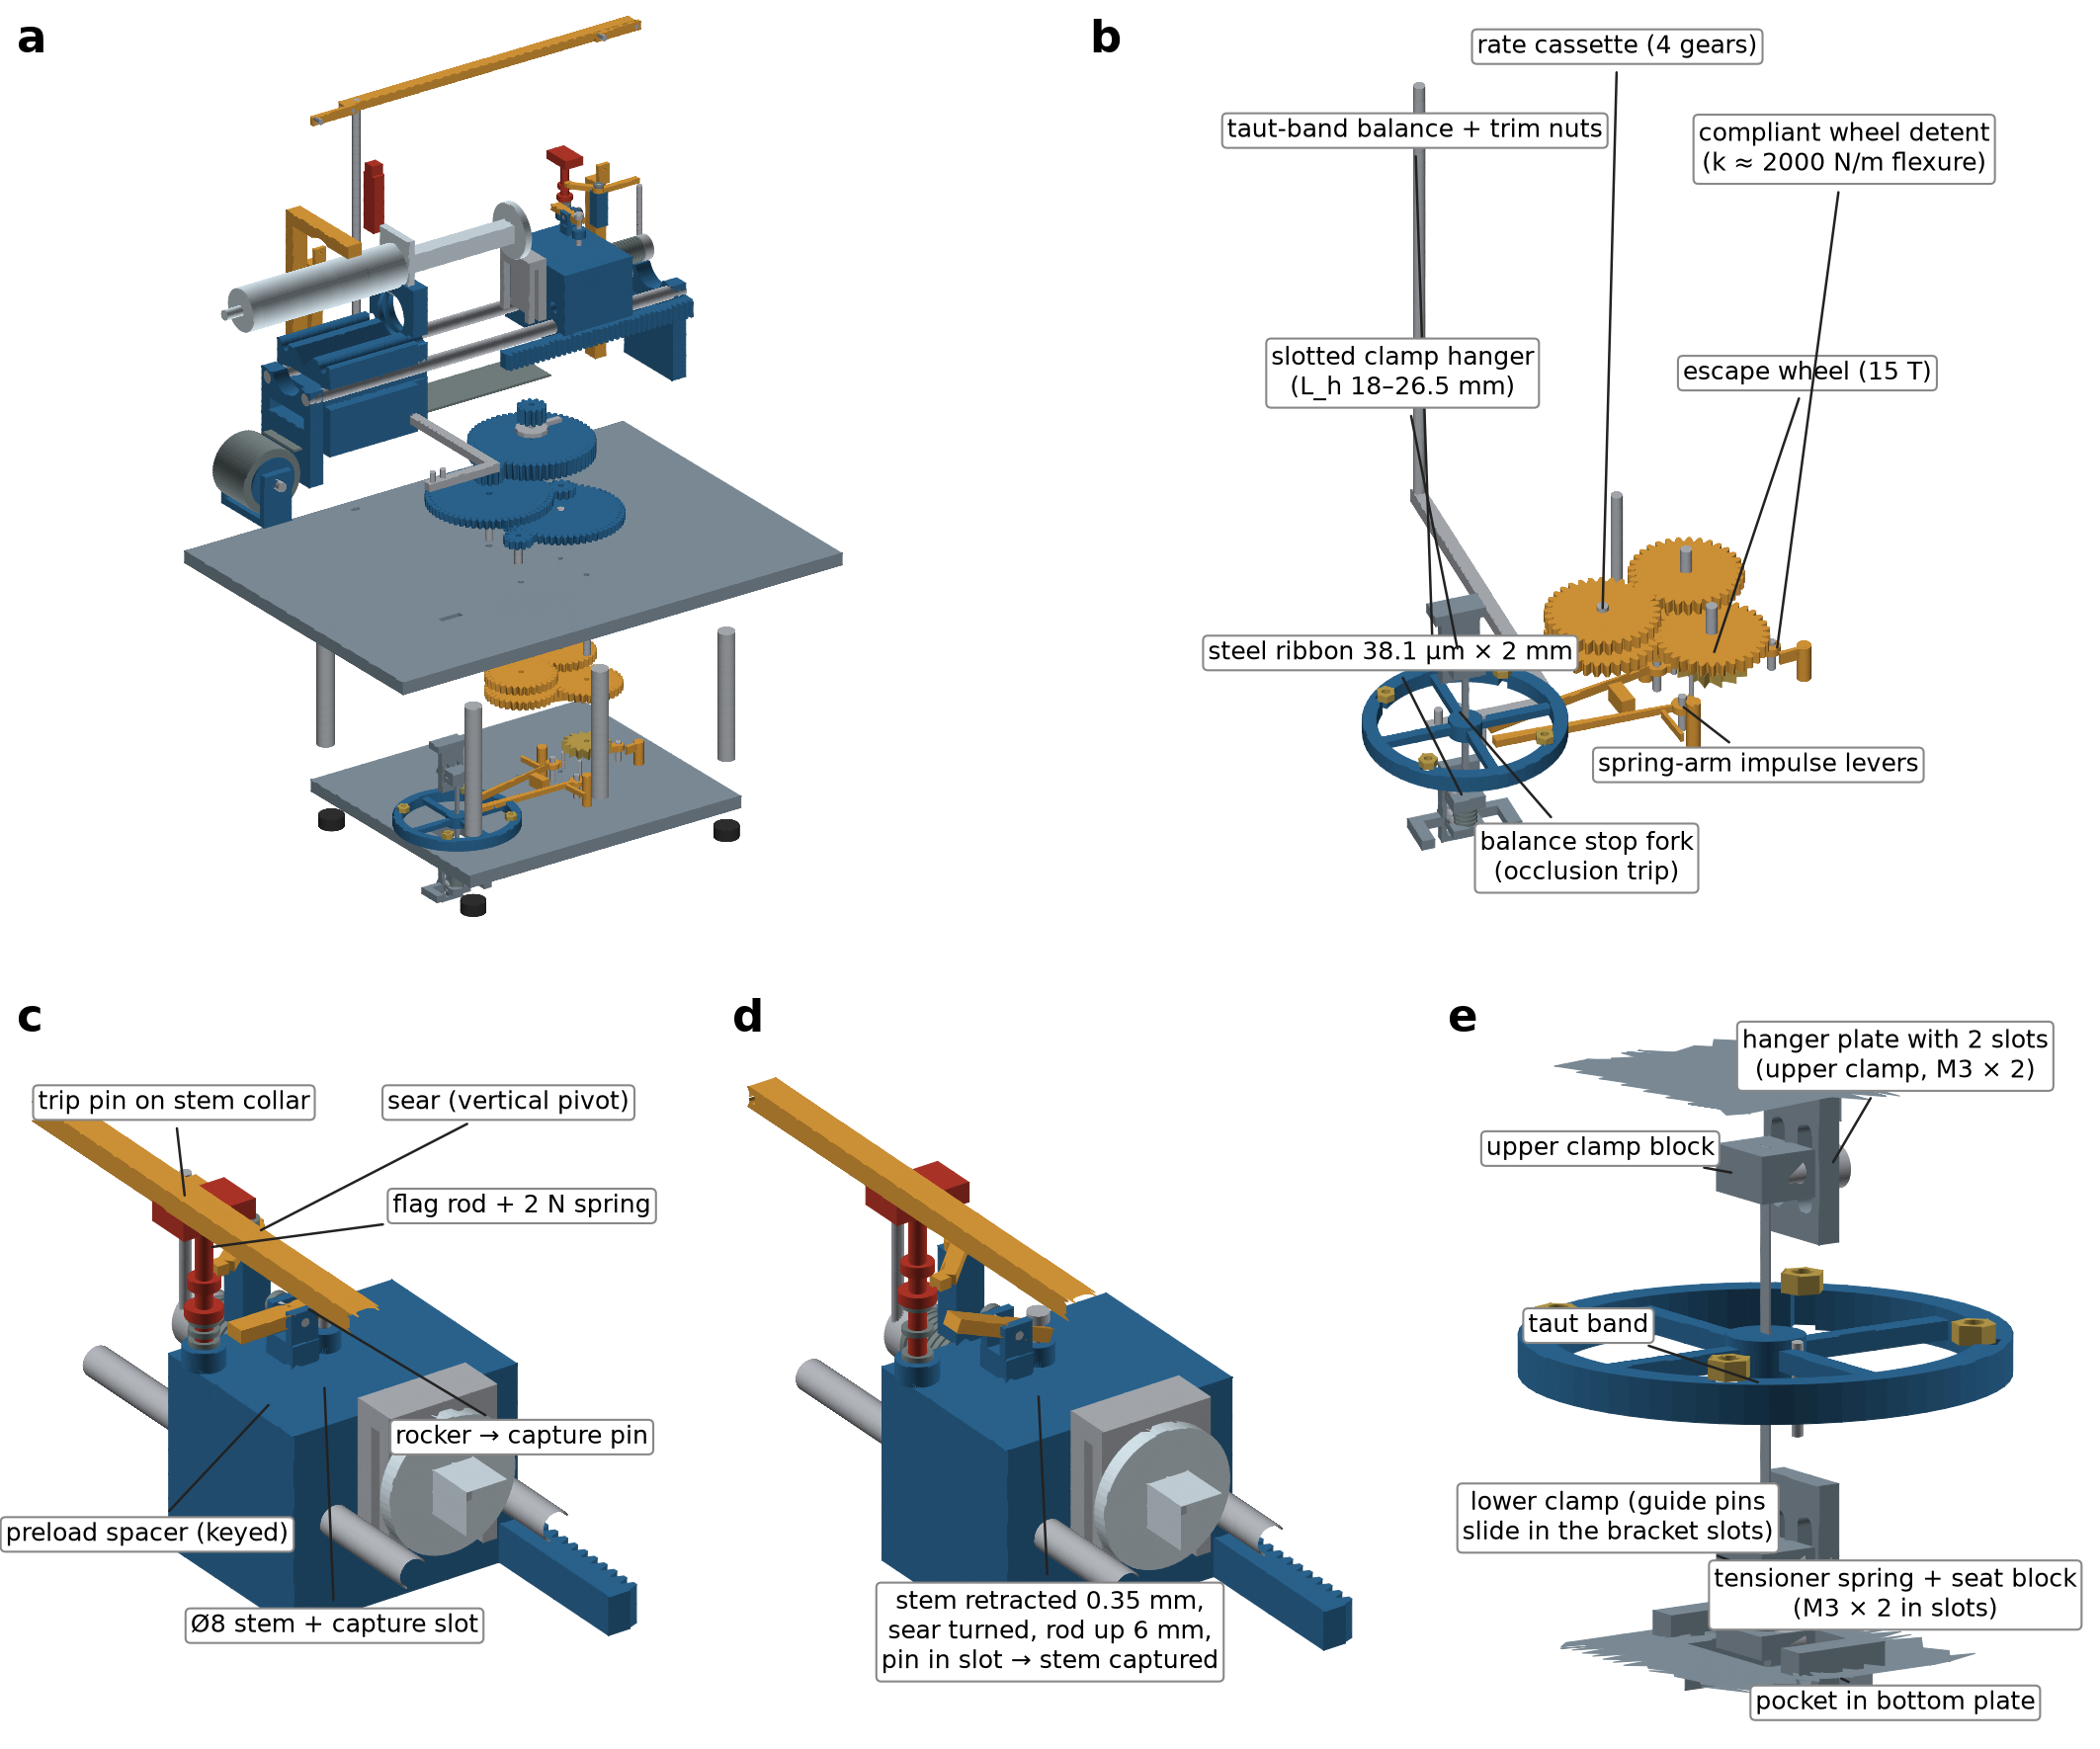
\includegraphics[width=\textwidth]{fig5.png}
\caption{\textbf{The complete 91-part assembly, including the snap-action occlusion trip and the adjustable band clamps, is fully modelled and interference-checked in twelve poses.} (a) Exploded view with parts separated along the vertical axis. (b) Escapement module with the deck removed: cassette, escape wheel, impulse arms, compliant wheel detent, balance with stop fork and slotted clamp hanger. (c) Occlusion trip on the carriage, armed: keyed spacer and trip spring behind the stem, trip pin on the end collar, sear on its vertical pivot holding the flag-rod collar, rocker and capture pin over the stem. (d) The same parts in the tripped pose: stem retracted \SI{0.35}{\milli\metre}, sear turned, flag rod up \SI{6}{\milli\metre}, capture pin in the stem slot, rail lifted. (e) Band clamps: slotted hanger plate with M3 screws for the upper clamp, slotted bracket with guide pins and screwed spring-seat block for the tensioner, both covering $L_h$ 18--\SI{26.5}{\milli\metre}.}
\label{fig:cad}
\end{figure}
\clearpage

\section{Discussion}
\ChronoFlow\ converts two precision-mechanics solutions---the constant-force escapement and the taut-band suspension---into a printable, electricity-free infusion driver whose predicted accuracy is limited by the syringe rather than by the fluid, the temperature, the back-pressure or the orientation of the device. Every safety function is mechanical and visible, and the rate is a physical object a nurse can hold and verify.

Several limitations follow from the fact that this is a design-and-simulation study. All performance figures are model predictions; the models are physics-based but unvalidated until the bench protocol below is executed. The balance quality factor in air and the efficiency of printed gear meshes are the least certain inputs; both were swept and both affect margin rather than rate. The spring-arm escapement geometry in the CAD is a representative embodiment whose latch, arm and detent proportions will need iteration on the bench, as horological escapements invariably do; the link by which the arm releases the detent, and the LOAD/RUN re-cocking of the flag rod and rocker, are described but not drawn. The mechanism-level analysis replaces the earlier constant-impulse assumption with derived values, but its contact parameters (latch friction, detent restitution) are inputs the bench must supply. Standalone reproduction of every figure was re-tested in this revision: the analysis scripts fall back to a bundled copy of the plotting helpers when the authoring environment is absent. The occlusion trip must be set per syringe size, which is a training requirement, and rates between cassettes require an additional printed cassette (any tooth set with sums of 66 can be made). The \SIrange{0.12}{1.16}{\micro\litre} pulsatility is small compared with a \SI{50}{\micro\litre} gravity-drip drop, but very low-rate inotrope infusions below \SI{0.5}{\milli\litre\per\hour} would be better served by a \SI{5}{\milli\litre} syringe.

\paragraph{Validation protocol.} (1) Measure the ribbon thickness with a micrometer (\SI{\pm 1}{\micro\metre}) and set the clamp post to the $L_h$ the stiffness model gives for that thickness; print the balance, clamp the ribbon and measure $f_0$ with a 240\,fps camera or light gate; set trims; measure $Q$ from the free-decay envelope; repeat band-horizontal, clamp-up and clamp-down (acceptance \SI{\pm 0.3}{\percent}). (2) Drive the escape wheel through the cassette with hanging weights emulating 17.6 and \SI{43}{\newton} excess (the \SI{60}{\milli\litre}-at-trip and \SI{5}{\milli\litre}-free-running corners of the operating map); verify re-cocking at the \SI{1}{\milli\litre\per\hour} cassette and constant amplitude by video tracking; tune arm flexure thickness. (3) Gravimetric flow test per IEC~60601-2-24 on a \SI{1}{\milli\gram} balance logged every \SI{30}{\second} for \SI{2}{\hour} per cassette; compute trumpet curves (acceptance: mean error \SI{\pm 5}{\percent}, trumpet \SI{\pm 10}{\percent} at \SI{2}{\minute}). (4) Repeat at 0, 100 and \SI{200}{mmHg} back-pressure and with \SI{10}{\percent} dextrose at 20 and \SI{37}{\celsius} (expected change $<\SI{1}{\percent}$). (5) Occlusion, for each syringe size with its cradle insert: measure plunger glide force on a load cell at the cassette speed (five syringes per lot), then clamp the line and record trip pressure against the predicted band (280--320 to 202--\SI{398}{mmHg} for \SI{60}{\milli\litre} to \SI{5}{\milli\litre}; shim the spacer if the lot's glide force differs from nominal by more than \SI{0.5}{\newton}), time to trip, the stem position after trip (captured, no creep), and bolus on release ($<\SI{0.2}{\milli\litre}$; this is the line-compliance bolus, since the captured stem contributes none). (6) Orientation and vibration (expected $<\SI{0.5}{\percent}$). (7) Seven-day continuous run and 200 load/unload cycles.

\section*{Data and code availability}
The parametric CAD (STEP, glTF, STL), the analysis code that reproduces every figure and number in this paper, the interference checker and the interactive viewer are provided in the accompanying repository.

\begin{thebibliography}{99}
\bibitem{autosyp} Juarez A, Maynard K, Skerrett E, Molyneux E, Richards-Kortum R, Dube Q, Oden ZM. AutoSyP: a low-cost, low-power syringe pump for use in low-resource settings. \emph{Am J Trop Med Hyg} 2016;95(4):964--969. doi:10.4269/ajtmh.16-0285.
\bibitem{asme2017} Guelig D, Bauer J, Wollen A, Schiller C, Sherman-Konkle J, Roche A, Weyrauch K, Eisenstein M. Design of a novel, adjustable flow rate, reusable, electricity-free, low-cost syringe infusion pump. \emph{ASME J Med Devices} 2017;11(4):041006. doi:10.1115/1.4037935.
\bibitem{asme2011} Sung C, Kamath RR, Cui Y, Ouyang C, Carstens E, Ramos RF, Oden ZM. Design of a novel mechanical syringe pump for neonatal care in low-resource settings. In: \emph{2011 IEEE Global Humanitarian Technology Conference}; 2011. p.~78--83. doi:10.1109/GHTC.2011.21.
\bibitem{han2021} Han W, Kim S, Shin S, Yang SY, Choi S, Shin JH. Wind-up precision pump for portable microfluidics. \emph{Sens Actuators B Chem} 2021;347:130592. doi:10.1016/j.snb.2021.130592.
\bibitem{park2024snb} Park SB, Shin JH. Fully 3D-printed, nonelectric, spring-powered syringe pump for operating microfluidic devices. \emph{Sens Actuators B Chem} 2024;405:135289. doi:10.1016/j.snb.2024.135289.
\bibitem{park2024hx} Park SB, Shin JH. Open-source spring-driven syringe pump with 3D-printed components for microfluidic applications. \emph{HardwareX} 2024;19:e00550. doi:10.1016/j.ohx.2024.e00550.
\bibitem{pooke2023} Pooke F, Payne M, Holder-Pearson L, Heaton D, Campbell J, Chase JG. Low-cost, low-power, clockwork syringe pump. \emph{HardwareX} 2023;16:e00469. doi:10.1016/j.ohx.2023.e00469.
\bibitem{denison} Denison EB. \emph{A Rudimentary Treatise on Clocks, Watches and Bells}. London: John Weale; 1850 (gravity escapement, ch.~on remontoires and gravity escapements).
\bibitem{timoshenko} Timoshenko SP, Goodier JN. \emph{Theory of Elasticity}, 3rd ed. New York: McGraw-Hill; 1970. \S\,109, torsion of a thin rectangular strip.
\bibitem{haringx} Haringx JA. The cross-spring pivot as a constructional element. \emph{Appl Sci Res} 1949;A1:313--332. doi:10.1007/BF02120338.
\bibitem{lewis} Lewis W. Investigation of the strength of gear teeth. \emph{Proc Engineers' Club of Philadelphia} 1893;10:16--23.
\bibitem{vogel} Vogel H. Das Temperaturabh\"angigkeitsgesetz der Viskosit\"at von Fl\"ussigkeiten. \emph{Phys Z} 1921;22:645--646.
\bibitem{iec} IEC 60601-2-24:2012. Medical electrical equipment --- Part 2-24: Particular requirements for the basic safety and essential performance of infusion pumps and controllers. Geneva: International Electrotechnical Commission; 2012.
\bibitem{iso7886} ISO 7886-1:2017. Sterile hypodermic syringes for single use --- Part 1: Syringes for manual use. Geneva: International Organization for Standardization; 2017.
\end{thebibliography}

\end{document}
